\documentclass{article}
\usepackage{proj1}
\usepackage{natbib}
\usepackage{amsmath}
%set spacing between lines (DO NOT CHANGE SPACING)
\linespread{1.25} %normally 1.25
\setlength{\parindent}{0cm}
\graphicspath{{Images/}}
%\underline{\smash{\beta}} makes underlining at the same distance
\usepackage{hyperref}

\hypersetup{
  colorlinks,
  allcolors=.,
  urlcolor=blue,
}
\usepackage{color}
\urlstyle{same}


%Definition of margins (DO NOT ALTER!)+

%\usepackage[a4paper, top=1in, left=1.0in, right=1.0in, bottom=1in, includehead, includefoot]{geometry} %Usually have top as 1in

%%%%%%%%%%%%%%%%%%%%%%%%%%%%%%%%%%%%%%%%%
% +++ ... +++ denotes something to be changed
%%%%%%%%%%%%%%%%%%%%%%%%%%%%%%%%%%%%%%%%%%
%Commands
\newcommand{\PDEsmall}[2]{\frac{\partial #1}{\partial #2}}
\newcommand{\PDE}[2]{\dfrac{\partial #1}{\partial #2}}
\newcommand{\folds}{(x_0,y_0)}
\newcommand{\st}{such that }
\newcommand{\wrt}{with respect to }
\newcommand{\vdp}{Van der Pol }
%%%%%%%%%%%%%%%%%%%%
\title{Fast Slow Dynamics - the van der Pol Oscillator}
\author{}
\date{October 2018}

\begin{document}

\maketitle

\section{Setup}
We wish to study the behaviour of the van der Pol oscillator using blow up. The van der Pol oscillator is a well-studied second order ODE used to model a variety of physical and biological phenomena. A position coordinate \(x(t)\) evolves according to the following equation. 
\begin{equation} \label{eq:vdP}\ddot{x}(t)-\mu\left(1-x^2(t)\right)\dot{x}(t)+x(t)=0   \end{equation}
Here, \(\mu \gg 1\) is a scalar constant. \par 

Currently, it doesn't resemble a anything like what we've seen in \cite{krupa2001}. To make it resemble a fast/slow system, we introduce a new variable. Let \(w=\dot{x}+\mu F(x)\) where \(F(x)=\frac{x^3}{3}-x\). Why have we chosen this function \(F\)? Notice that \(F'(x)=-(1-x^2)\), our nonlinear term in Equation \ref{eq:vdP}. Differentiating \(w\) we obtain
\begin{align*}
    \dot{w}&=\ddot{x}+\mu\od{}{x}\left(\frac{x^3}{3}-x\right)\od{x}{t}\\
    & =\ddot{x}+\mu(x^2-1)\dot{x}\\
    &= -x
\end{align*}
Here, the last equality follows from the van der Pol equation. We now have a two dimensional system.
\[\begin{cases} \dot{x}=w-\mu F(x)\\
 \dot{w}=-x\end{cases}\]
 Let \(y=\frac{w}{\mu}\). Then
 \[\begin{cases} \dot{x}=\mu\left(y-F(x)\right)\\
 \dot{y}=-\frac{x}{\mu}\end{cases}\]
We will pause here although it doesn't look quite right and do a phase plane analysis to better understand the behaviour of the system. Setting each equation equal to zero in turn gives nullclines of \(x=0\) and \(y=F(x)\). 

+++ PHASE PLANE ANALYSIS +++

+++ New transformation to fast/slow system +++


Fast System:
\begin{equation}\label{fastsystem}
    \begin{cases} x'=y-F(x)\\
    y'=-\epsilon x
    \end{cases}
\end{equation}


Slow system:
\begin{equation}\label{slowsystem}
    \begin{cases} \epsilon \dot{x}=y-F(x)\\
    \dot{y}=-x
    \end{cases}
\end{equation}

\subsection{Fold Points}\label{Fold Points}
The fold points are $(x_0^+,y_0^+)=(1,-\dfrac{2}{3})$ and $(x_0^-,y_0^-)=(-1,\dfrac{2}{3})$
\begin{figure}[h]
    \centering
    %\includegraphics{}
    \caption{Our Manifold $f(x,y,\epsilon)$}
    \label{fig:my_label}
\end{figure}

\subsection{Non-degeneracy}
Now that we have established our fast-slow systems (Equation \ref{fastsystem} and \ref{slowsystem}) we need to check our non-degeneration conditions \citep{krupa2001}. 
%Before proceeding it is prudent to note that the nondegeneracy conditions will be opposite for the case where $(x_0,y_0)=(x_0^+,y_0^+)$ to satisfy our system.
Now we first check that $ \pd{^2f}{x^2}(x_0,y_0,0)\neq 0$ then we have,
\begin{equation}
    \pd{^2}{x^2}(y-\dfrac{x^3}{3}-x)=-2x,
\end{equation}
which we can evaluate at our fold points (Section \ref{Fold Points}) to give,
\begin{equation} 
    \begin{cases}
            &\pd[2]{f}{x}(x_0^+,y_0^+,0)=2<0\\
            &\pd[2]{f}{x}(x_0^-,y_0^-,0)=2>0.
    \end{cases}
\end{equation}
Then we can consider that $\pd{f}{y}(x_0,y_0)\neq 0$. We show this by the following,
\begin{align}
        &\pd{f}{y}(x_0^+,y_0^+,0)=1\\
        &\pd{f}{y}(x_0^-,y_0^-,0)=1.
\end{align}
Lastly we need to consider that $g(x_0,y_0,0)\neq 0$. This is easily seen as we find that $g(x_0,y_0,0)=\pm 1$ for our two fold points. From here we are can now consider our transformation.


\section{Charts}\label{sec: charts}
include picture from the book \begin{figure}[h!]
    \centering
    %\includegraphics{}
    \caption{Charts}
    \label{fig: charts}
\end{figure}

\section{Transformation}

\citet{krupa2001} discusses why we should make a transformation for our system. We find that if we map $\folds=(0,0)$ we are then able to simplify our non-degeneracy conditions - as shown in Equation \ref{non-degeneracy} \citep{krupa2001}.
\begin{equation}
    \begin{cases}
        &\folds=(0,0)\\
        &\pd{^2f}{x^2}(0,0,0)>0\\
        &\pd{f}{y}(0,0,0)<0
    \end{cases} 
    \label{non-degeneracy}
\end{equation}

\subsection{Mapping Transformation}\label{sex: mapping}
To be able to continue with our analysis we should consider the transformations. We will first only consider the case for our fold point at $(x_0^+,y_0^+)=(1,-\dfrac{2}{3})$. We wish to map $(x,y)\to (1-\Tilde{x},\Tilde{y}-\frac{2}{3})$ which reflects and translates our system \st our fold points are now mapped to $(0,0)$ - Figure \ref{fig: Transformed System}. 

\begin{figure}[h]
    \centering
    %\includegraphics{}
    \caption{Our transformed system.}
    \label{fig: Transformed System}
\end{figure}
Now that we have made our transformation we can check our non-degeneracy conditions. However, before we continue we should check that our the sign of the derivative is conserved through the transformation. We can do this by using the chain rule as follows, 

\begin{equation}
    \od{x}{t}=\od{\Tilde{x}}{x}\od{x}{t}=-\od{\Tilde{x}}{t}. \label{chain rule}
\end{equation}
Now using Equation \ref{chain rule} and our new mapping ( $(x,y)\to (1-\Tilde{x},\Tilde{y}-\frac{2}{3})$) we are able to define our new Fast System in the following way, 
\begin{equation}
    \begin{cases}
        x'=-y+x^2-\dfrac{(x)^3}{3}\\
        y'=\epsilon(x-1)
    \end{cases}
    \label{eq: Fast System}
\end{equation}
where we note that we have dropped the tilde on $x \ \text{and} \ y$ for convenience. \\

\subsection{Non-degeneracy Conditions}
\begin{equation}
    \begin{cases}
        &\folds=(0,0)\\
        &\pd[2]{f}{x}(0,0,0)>0\\
        &\pd{f}{y}(0,0,0)<0
    \end{cases} 
    \tag{\ref{non-degeneracy}}
\end{equation}
Now that we have constructed our transformed system, we are now able to check our non-degeneracy conditions - Equation \ref{non-degeneracy}. It is clear to see that $\folds=(0,0)$ by the mapping we defined in Section \ref{sex: mapping}. Following this we are able to check our other non-degeneracy conditions conform to our new mapping. The differentiation is easily seen from Equation \ref{eq: Fast System} which yields that $\pd[2]{f}{x}(0,0,0)=2>0$ and $\pd[1]{f}{y}(0,0,0)=-1<0$, confirming our assumptions.


\subsection{Reduced Dynamics}
The next progression for our system is to consider the reduced dynamics within our system. To do this we consider Equation \ref{slowsystem} and take the $\epsilon\to0$ which yields the following system,
\begin{subequations}
    \begin{align}
    &0=f(x,y,0)=-y+x^2-\dfrac{x^3}{3}\\
        &\dot{y}=g(x,y,0)=0 \label{eq: reduced g}
    \end{align}
\end{subequations}
which is known as the slow subsystem \citep{Kuehn}. We are then able to compute the reduced flow by computing  \citep{krupa2001},
\begin{equation}
    \phi_x(x)\dot{x}=g(x,\phi(x),0),\text{ for }y=\phi(x).
    \label{eq: general reduced}
\end{equation}
We find that $\phi(x)=x^2-\dfrac{x^3}{3}$ where the derivative \wrt $x$ gives $\phi_x(x)=2x-x^2$. Now it is clear that we will have a singularity at $x=0$, by Equation \ref{eq: general reduced}, thus we will find that our system blows up ($\dot{x}\to\infty$) which motivates the process that will follow. \\ \\
%note that the sign g(0,0,0) determines the flow direction 
%g(0,0,0)<0 as expected in our example.
After finding our reduced system we are able to determine the way in which it flows by considering the sign of $g(0,0,0)$. We see from Equation \ref{eq: reduced g} that $g<0$ then we have that our flow is directed towards the fold points $(0,0)$. To continue with our analysis we first need to define Fenichel's theorems.

\subsection{Fenichel and Standard Theory}
\textbf{THEOREM}

\subsection{Extended System}
Now that we have established the above theorems then we need to consider the extended system \st $\epsilon'=0$, thus $\epsilon=\text{\textit{const}}$. By considering this system we will be able to consider a blow up (magnification) around our fold point in three dimensions.  
\begin{figure}[h]
    \centering
%    \includegraphics{}
    \caption{Blown up system}
    \label{fig: blow up}
\end{figure}
From Figure \ref{fig: blow up} we can consider the stability of our fold point. To do this we are able to establish the following determinant,
\begin{equation} 
    A=\begin{vmatrix} 2x-x^2-\lambda & -1&0 \\ 0 & -\lambda&0\\0&0&-\lambda \end{vmatrix}=\lambda^2(2x-x^2-\lambda).
    \label{eq: Eigenvalues}
\end{equation}
However, a far easier approach is to note that our matrix is an upper triangular matrix which we can take the eigenvalues directly from Equation \ref{eq: Eigenvalues} \st $(\lambda_1.\lambda_2,\lambda_3)=tr(A)$. Then we can clearly see that for our fold points $\lambda_i=0 \ \text{for} \ i=1,2,3$ and for any $x\neq0$ we have $\lambda_1=x(2-x)$ and $\lambda_2=\lambda_3\equiv0$. As a result we can see that we are forced to blow up our system around our fold point as our steady states are non-hyperbolic whereas outside of this we find that we have one hyperbolic steady state.
%Now we can see that we have three non-hyperbolic eigen values when we consider our system at (0,0,0), 


\subsubsection{Canonical Form}
Now that we have established our reduced system we are able to rewrite it in canonical form - Equation \ref{eq: canonical}.
\begin{equation}
    \begin{aligned}
        &x'=-y+x^2-\frac{x^3}{3}=-y+x^2+h(x) \\
        &y'=\epsilon(x-1)
    \end{aligned}
    \label{eq: canonical}
\end{equation}
There is ample reasoning for doing this. This is because we find that the canonical form has been studied in great detail allowing us to make comparisons and to avoid excess computation. This then allows us to follow an analogous approach to the many papers associated with this topic - as seen in \citet{krupa2001} paper on Extending Geometric Singular Perturbation Theory.


\section{Blow-ups in our System}\label{sec: VDP Blowup}
%++++Rename chapter: 'The Blow-Up Method'++++++++
\subsubsection{Extended System} \label{sec: extended sys blowup}
++++ weave in +++++++++
The canonical system (Equation \ref{eq: canonical}) is then extended to three dimensions by considering $\epsilon'=0$. 
\begin{equation} \label{extended FS}
\begin{aligned}
&x'=-y+x^2+h(x) \\
&y'=\epsilon(x-1)\\
&\epsilon'=0.
\end{aligned}
\end{equation}




In order to apply the Blow-Up Method to the fold point at the origin, we focus on a neighbourhood $U$ around the fold point $(0,0)$. 
The neigbourhood $U$ is small enough, such that $g(x,y, \epsilon) \neq 0$ in $U$, and we can define sections in $U$, as follows:
\begin{align*}
&\Delta ^{in} = \{ (x, \rho^2), x \in I \} \\
&\Delta ^{out} = \{ (\rho, y), y \in \mathbf{R} \},
\end{align*}
where $I \subset \mathbf{R}$. Now $\Delta^{in}$ is transverse to $S^a$, while $\Delta^{out}$ is transverse to the fast flow. This enables us to monitor the incoming trajectories from the attracting branch of $S$ and the trajectories leaving $U$ in the direction of the fast flow.
Then a function $\pi : \Delta^{in} \to \Delta^{out}$ can be defined, called the transition map, which describes how the trajectories passing through $\Delta^{in}$ are mapped onto the outgoing flow in $\Delta^{out}$.  
The following theorem describes the behaviour of the flow under $\pi$.
% and a sketch of the proof will be given at the end of this section: ++++last statement not precise+++

\begin{theorem}[\citealp{krupa2001}] \label{transition map theorem}
Under the assumptions made in this section, there exists $ \epsilon_0 >0$ such that the following assertions hold for $\epsilon \in (0, \epsilon_0]$:\\
1. The manifold $S_\epsilon^a$ passes through $\Delta^{out}$ at a point $(\rho, h(\epsilon))$, where $h(\epsilon) = O(\epsilon^{2/3})$.\\
2. The transition map $\pi$ is a contraction with contraction rate $O(e^{-c/\epsilon})$, where $c$ is a positive constant.
\end{theorem}
This means that the trajectories that enter $U$ through $\Delta^{in}$, will be funneled into a smaller section of $\Delta^{out}$ and therefore we are guaranteed to observe the trajectories that enter through $\Delta^{in}$ in $\Delta^{out}$. Now we are in the position to describe the method of Blow-Up Transformations in the neighbourhood $U$.

\subsection{Coordinate Transformation and Charts} \label{sec:transform blowup}
We first need to transform the extended system (\ref{extended FS}) with respect to the time variable and the space variables. This coordinate transformation is called the Blow-Up Transformation because the degenerate fold point $(0,0)$ is regarded as a sphere of radius $r=0$. By rescaling the space variables with respect to different weights of $r$,
\begin{subequations}
    \begin{align}
        &x=\Bar{r}\Bar{x}  \label{sys: blow up trans x}\\
        &y=\Bar{r}^2\Bar{y} \label{sys: blow up trans y}\\ 
        &\epsilon=\bar{r}^3\bar{\epsilon} \label{sys: blow up trans z},
    \end{align}  
    \label{sys: blow up trans}
\end{subequations}
we find that we are able to carry out further analysis, as will follow.
%+++++ If time and space permit, an analysis of the space B and coordinate map would be good... p.291 krupa++++
%A reasonable question to consider is why do we note consider spherical polar coordinates. The reasoning behind this is because we are looking to maximise our computational efficiency so we will proceed in cartesian coordinates.
Instead of analysing the sphere in spherical polar coordinates, which might seem the most obvious choice of method,  the rest of this analysis is done using charts, described below (see \citet{needam} for the construction of charts on a sphere). This method turns out to be a more natural choice for this problem and maximises computational efficiency.
\begin{figure}[h!]
	\centering
	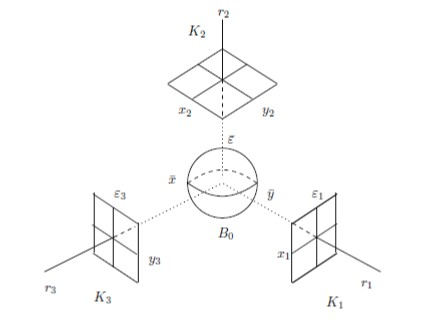
\includegraphics[height=5cm,width=7cm]{Images/charts-ball}
	\caption{Three charts mapping different sections of our blow up \citep{krupa2001}.}
	\label{fig:chartDiagram}
\end{figure}
In terms of the blown up fold point, a sphere denoted by $B$, charts are projections of regions of $B$ onto a two dimensional plane. 
We introduce three charts $ K_1,K_2,$ and $K_3 $. Chart $K_2$ is the two dimensional projection covering the upper half plane of $B$. However, as points on the equator of $B$ are approached on $K_1$, the point tends to infinity. These regions however, are of immense interest, since they are points of incoming and outgoing trajectories. As a consequence, charts $K_1$ and $K_3$ are introduced, covering the regions of interest on the equator of the fold point. 
%This is represented in Figure ++++++ (blow up figure)++
%The points that are relevant to the analysis of the dynamics are shown in Figure (+++insert figure 2.2 p,293+++++). (More description potentially)
The charts are defined by setting each of the variables of the extended system to $1$ in turn, giving $ \bar{y}=1, \ \bar{\epsilon}=1, \ \bar{x}=1 $. Substituting these into Equations (\ref{sys: blow up trans x}), (\ref{sys: blow up trans y}) and (\ref{sys: blow up trans z}) respectively gives, 
\begin{subequations} \label{ sys: K1K2K3}
	\begin{align}
	&x=r_1x_1, \ y=r_1^2, \ \epsilon=r_1^3\epsilon_1, \label{sys: K1}\\
	&x=r_2x_2, \ y=r_2^2y_2, \ \epsilon=r_2^3 \label{sys: K2}\\
	&x=r_3, \ y=r_3^2y_3, \ \epsilon=r_3^3\epsilon_3\label{sys:K3}
	\end{align}
\end{subequations}
where $ (x_i,r_i,\epsilon_i)\in\mathbf{R}^3 $ for $ i=1,2,3 $, and the equations correspond to the charts in numerical order \citep{krupa2001}. 
With this setup, we can consider the individual charts in turn, analyse the dynamics on the individual charts, and then join the gathered information into a global view on the dynamics in $U$.
We start with $K_2$,  because it holds the most information and the flow is the analysed more readily than in the other two charts. 
The remaining question is how the transition between the three charts and the connection to the global dynamics is made after finishing the individual analysis.
This is done via a coordinate change, derived by using Equations \ref{ sys: K1K2K3} and \ref{sys: blow up trans}, and the results are summarised in the following Lemma:
\begin{lemma} \label{coord. change}
Let $\kappa_{12}$ denote the change of coordinates from $K_1$ to $K_2$. Then $\kappa_{12}$ is given by \\
\begin{equation*}
x_2 = x_1 \epsilon_1^{-1/3},  y_2 = \epsilon_1^{-2/3}, r_2= r_1\epsilon_1^{1/3},
\end{equation*}
for $\epsilon_1 >0$,
and $\kappa_{12}^{-1}$ is given by
\begin{equation*}
x_1 = x_2y_2^{-1/2}, r_1 = r_2 y_2^{1/2}, \epsilon_1= y_2^{-3/2},
\end{equation*}
for $y_2>0$.
Let $\kappa_{23}$ denote the change of coordinates from $K_2$ to $K_3$. Then $\kappa_{23}$ is given by
\begin{equation*}
r_3 = r_2x_2, y_3= y_2x_2^{-2}, \epsilon_3 = x_2^{-3}, \label{eq:kappa23}
\end{equation*}
for $x_2>0,$
and $\kappa_{23}^{-1}$  is given by
\begin{equation*}
x_2 = \epsilon_3^{-1/3}, y_2 = y_3\epsilon_3^{-2/3}, r_2= r_3 \epsilon_3^{1/3},
\end{equation*}
for $\epsilon_3>0$.
\end{lemma}

Furthermore, transition maps $\Pi_i, i \in 1,2,3$  are defined in each section, describing how the trajectories coming in and out of each chart. These are combined in the final part of this section to give the proof of Theorem \ref{transition map theorem}, and to relate the results of the blow up method back to the original transition map $\pi$.
\newpage
\subsection{Dynamics in \texorpdfstring{$K_2$}{K2}} \label{sec: VDP K2}
\begin{figure}[h!]\centering
	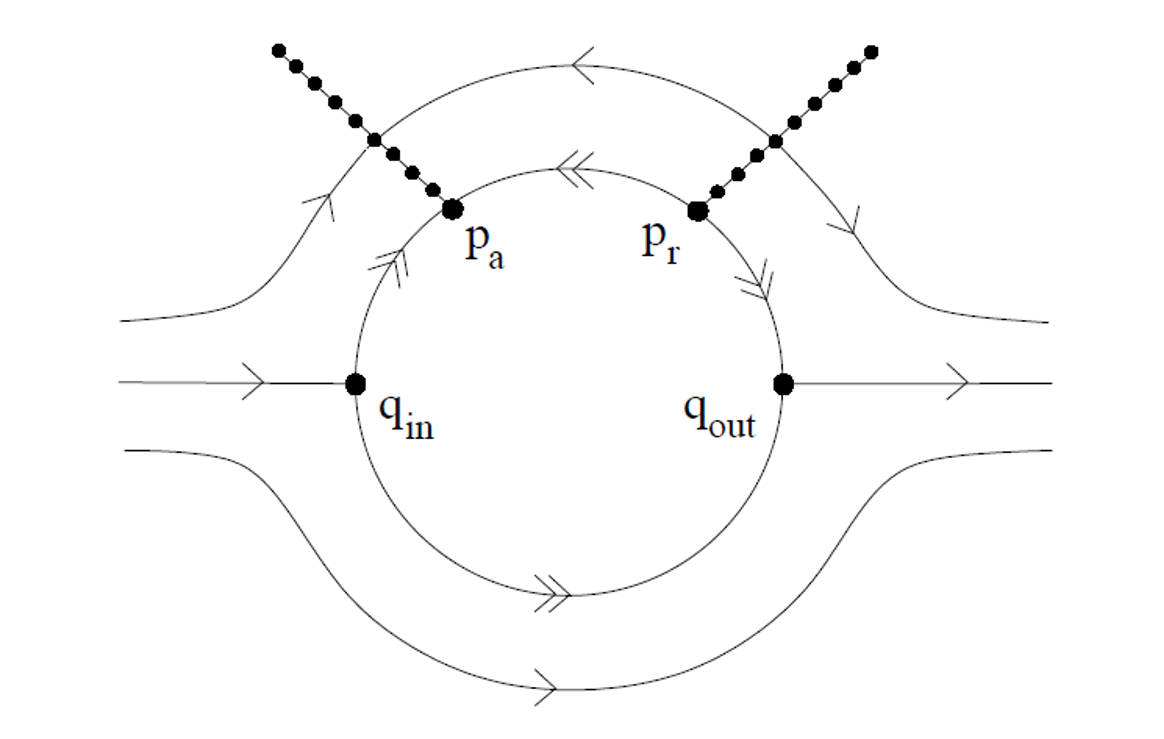
\includegraphics[height=4cm,width=6cm]{Images/Dynamics_in_Chart_2}
	\caption{Phase portrait for chart 2 \citep{krupa2001}.}
	\label{fig: chart 2 fig}
\end{figure}
To be able to consider chart $ K_2$, the transformation presented in Equation \ref{sys: K2} is applied to the extended system (\ref{extended FS}). Furthrmore,a time rescaling ($ t_2=r_2t $) is applied to desingularise the system. This results in:
\begin{equation}
	\begin{aligned}
		&\od{}{t}(r_2x_2)=r_2^2\od{x_2}{t}=-y_2+x_2^2-\dfrac{x_2^3r_2}{3},\\
		&r^3_2y'_2=r^3_2(-1+r_2x),\\
		&r'_2=0,
	\end{aligned}
\end{equation}
noting that $ \od{r}{t_2}=\od{t}{t_2}\od{r}{t}=\frac{1}{r_2}\od{r_2}{t} $ .  Now dividing through by $ r^2_2 $ and $ r^3_2 $ respectively for each equation and grouping $O(r_2)$ terms we get,
\begin{equation}
	\begin{aligned}
		&x'_2=x^2_2-y_2+O(r_2),\\
		&y'_2=-1+O(r_2),\\
		&r'_2=0.
	\end{aligned}
\end{equation}
Then, considering $r_2=0$ and neglecting the $O(r_2)$ terms results in,
\begin{equation} \label{Riccati}
	\begin{aligned}
		&x'_2=x^2_2-y_2,\\
		&y'_2=-1,\\
	\end{aligned}
\end{equation}
which are the well known Riccati equations- see \citet{Riccati}.
Some known results about the Riccati equations can be summarised as follows:


\begin{prop}[\citealp{krupa2001}]\label{Riccati Prop} 
The Riccatti equation (\ref{Riccati}) has the following properties:
\begin{enumerate}
\item Every orbit has a horizontal asymptote $y=y_r$, where $y_r$ depends on the orbit such that $x \to \infty$ as $y$ approaches $y_r$ from above.
\item There exists a unique orbit $\gamma_2$, which can be parameterized as $(x,s(x)), x \in \mathbf{R}$ and is asymptotic to the left branch of the parabola $x^2 - y = 0$, for $x \to - \infty$. The orbit $\gamma_2$ has a horizontal asymptote $y= - \Omega_0 <0$, such that $x \to \infty$ as $y$ approaches $-\Omega_0$ from above.
\item The function $s(x)$ has the asymptotic expansions
\begin{align*}
s(x) &= x^2 + \frac{1}{2x} + O\left( \frac{1}{x^4} \right), x \to -\infty,\\
s(x) &= -\Omega_0 + \frac{1}{x} + O\left( \frac{1}{x^3} \right), x \to \infty.
\end{align*}
\item All orbits to the right of $\gamma_2$  are backward asymptotic to the right branch of the parabola $x^2-y=0$.
\item All orbits to the left of $\gamma_2$ have a horizontal asymptote $y=y_l>y_r$, where $y_l$ depends on the orbit, such that $x \to -\infty$ as $y$ approaches $y_l$ from below.
\end{enumerate}
\end{prop}

The solutions to the Riccati equations, described in Proposition \ref{Riccati Prop}, are displayed in Figure. Note that the equation $x^2 - y=0$ is locally the critical manifold $S$ close to the fold point.%+++a bit wavy argument+++
The orbit $\gamma_2$, corresponds to the global trajectory $\gamma$, of the full system, which is the candidate trajectory connecting the slow flow on $S^a$ entering $U$ through $p_a$ to the fast fibres, exiting $U$ through $q_{out}$ - described by Figure \ref{fig: Ricatti Sol}. 
\begin{figure}[h!]\centering
	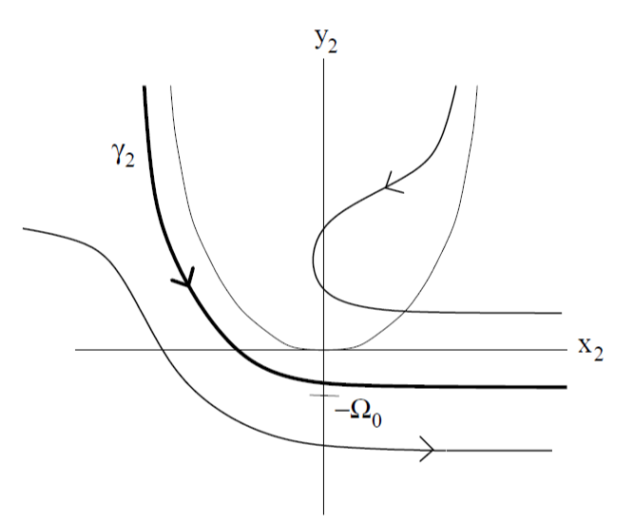
\includegraphics[height=6cm,width=6cm]{Images/Dynamics_in_K2}
	\caption{Ricatti solution for chart 2 \citep{krupa2001}.}
	\label{fig: Ricatti Sol}
\end{figure}
 
%(++++++refer back to figure  2.2 in krupa+++++++++)
This leads to the conclusion that if we can connect $\gamma_2$ to $p_a$  through $K_1$ and to $q_{out}$ through $K_3$, the global $\gamma$ can be constructed using Lemma \ref{coord. change}.
This motivates the analysis of $K_1$ and $K_3$.
In order to connect the dynamics on $K_2$ to that on the other charts, we need to define local inflow and outflow sections, similar to $\Delta^{in}$ and $\Delta^{out}$ in the full system.
Then we can follow trajectories that get mapped by $\Pi_2$, again analogous to $\pi$ in the full system, from a section $\Sigma^{in}_2$ to $\Sigma^{out}_2$.
The section are defined as follows. For $\delta>0$, we have:
\begin{align*}
\Sigma^{in}_2= \{ (x_2,y_2,r_2): y_2= \delta^{-2/3} \},\\
\Sigma^{out}_2 = \{ (x_2,y_2,r_2): x_2 = \delta^{-1/3} \}.
\end{align*}
Then the transition map $\Pi_2$ can be defined and the results are summarised as follows:
\begin{prop}[\citealp{krupa2001}]
The transition map $\Pi_2$ has the following properties:
\begin{enumerate}
\item
\begin{align*}
\Pi_2(q_0)= (\delta^{-1/3}, - \Omega_0 + \delta^{1/3} + O(\delta), 0)
\end{align*}
\item A neighbourhood of $q_0$ is mapped diffeomorphically onto a neighbourhood of $\Pi_2(q_0)$.
\end{enumerate}
\end{prop}
 
This is sufficient information to now consider the dynamics on $K_1$.

\subsection{Dynamics in \texorpdfstring{$K_1$}{K1}}\label{sec:dynamics-in-texorpdfstringk1k1} 
The coordinate transformation (\ref{sys: K1}) is applied to the extended system (\ref{extended FS}), 
\begin{align*}
\frac{d(r_1x_1)}{dt_1} \frac{dt_1}{dt} = -r_1^2 + r_1^2x_1^2 - \frac{1}{3}r_1^3x_1^3,\\
\frac{dr_1^2}{dt_1}\frac{dt_1}{dt}= 2r_1^2r_1' = r_1^3 \epsilon_1 (-1 +r_1 x_1),\\
\frac{d(r_1^3 \epsilon_1)}{dt_1}\frac{dt_1}{dt}= (3r_1^2\epsilon_1 + r_1^3 \epsilon_1') r_1 = 0.
\end{align*}
Dividing through by $\frac{dt_1}{dt}=r_1$ and replacing the expressions for $\epsilon_1'$ and $r_1'$ with their expressions in terms of the variables, results in the full system in terms of $K_1$. Note that the equation for $\epsilon'$ is found by rearranging the third equation above. 
\begin{align*}
x_1' &= -1 +x^2 + \frac{1}{2} x_1 \epsilon_1 + \left( - \frac{1}{2} \epsilon_1 x_1^2r_1 - \frac{1}{3} x_1^3 \right)\\
r_1' &= \frac{1}{2} r_1 \epsilon_1( -1 + r_1 x_1)\\
\epsilon_1' &= \frac{3}{2} \epsilon_1^2 ( 1- r_1x_1),
\end{align*}
and grouping terms in $r_1$ results in the standard form:
\begin{equation}
\begin{aligned} \label{K1systemfull}
x_1' &= -1 +x^2 + \frac{1}{2} x_1 \epsilon_1 +O(r_1)\\
r_1' &= \frac{1}{2} r_1 \epsilon_1( -1 + O(r_1))\\
\epsilon_1' &= \frac{3}{2} \epsilon_1^2 ( 1- O(r_1)).
\end{aligned}
\end{equation}

The system (\ref{K1systemfull}) has two invariant planes, that are somewhat equivalent to the notion of a nullcline. This tell us that the rate of change for our confidantes, $ r_1 $ and $ \epsilon_1 $ is constant for r$ _1=0 $ and $\epsilon_1=0$. If we substitute $r_1=0$ or $\epsilon_1=0$ into (\ref{K1systemfull}), the $r_1$ or $\epsilon_1$ equation respectively, are both zero, and there is only a two dimensional system left to consider. These two subspaces of (\ref{K1systemfull}) will be analysed below. Furthermore, the subspace where $r_1=0$ and $\epsilon_1=0$, is one dimensional, an invariant line, where the subspaces $r_1=0$ and $\epsilon_1=0$ cross.
The following analysis is displayed in Figure \ref{fig:k1chart}, illustrating the dynamics on $K_1$.
%\begin{figure}[h!]
%	\centering
%	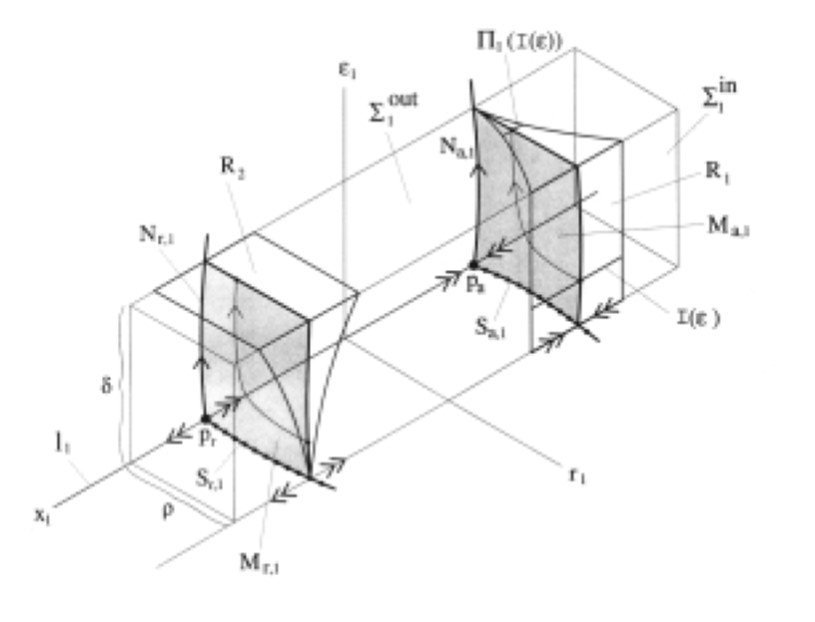
\includegraphics[width=7cm, height=7cm]{Images/K1Chart}
%	\caption{Dynamics in chart 1 \citep{krupa2001}
%	\label{fig:k1chart}
%\end{figure}
\begin{figure}[h!]
	\centering
	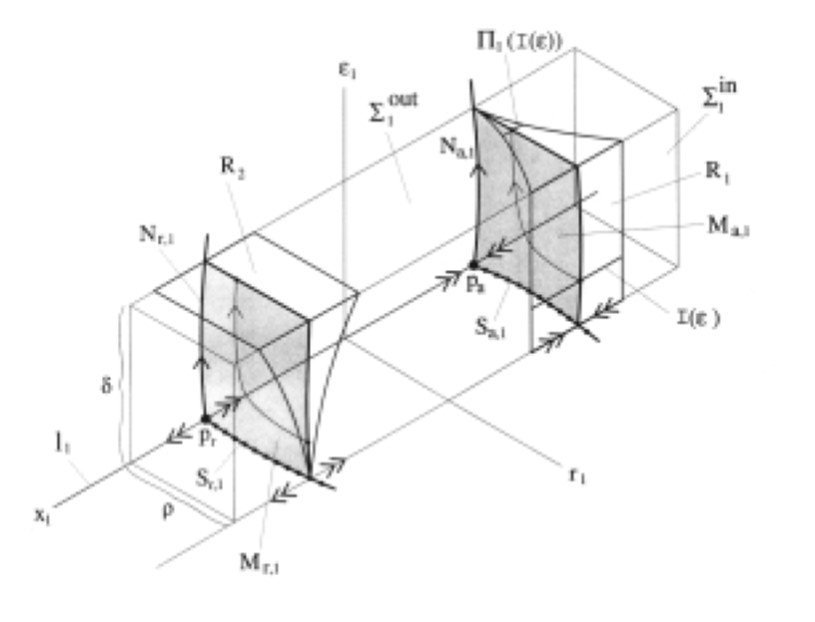
\includegraphics[height=7cm,width=7cm]{Images/K1Chart}
	\caption{Dynamics in chart 1 \citep{krupa2001}}
		\label{fig:k1chart}
\end{figure}\newpage


The invariant line, satisfying $r_1=0$ and $\epsilon_1=0$ is given by $l_1= -1 +x^2$. From this it is easily deduced that the two equilibrium points are where $l_1=0$, which is at $x=\pm1$. Therefore, the points $p_a$ and $p_r$ are defined as $p_a= (-1,0,0)$ and $p_r=(1,0,0)$. The flow on $l_1$ is attracted to $p^a$ and repelled by $p^r$, which is easily observed from the form $l_1$ takes or from a formal stability analysis of the one dimensional system. The eigenvalues of $l_1$ are found  by considering $l'_1 - \lambda = 2x - \lambda= 0 $ which gives that $\lambda = \pm 2$ at the respective equilibria. Then we expect the behaviour of the flow on the two invariant planes to be influenced by the two equilibria and the dynamics on $l_1$.
Consider the plane $\epsilon_1=0$. The system (Equation \ref{K1systemfull}) becomes
\begin{equation}
\begin{aligned} \label{epsilon0sys}
x_1' &= -1 +x_1^2 - \left( \frac{1}{3}r_1x_1^3 \right)\\
r_1' &= 0.
\end{aligned}
\end{equation}
This system has equilibria at $x= \pm1$, for $r_1=0$, as before, however, for each constant value of $r_1$, we get a different equilibrium of the system (\ref{epsilon0sys}). This forms a curve of equilibria, which can be recognised as $S^a_1$ connected to $p_a$ and $S^r_1$ connected to $p_r$, of the critical manifold, transformed into $K_1$ - this follows from the Implicit Function Theorem, see Figure \ref{fig: chart 2 fig}. The additional eigenvalue, corresponding to the $r_1$ equation, is $\lambda=0$. However, at each of the equilibria of this system, and specifically at $p_a$ and $p_r$ we have normal hyperbolicity, due to the coordinate transformation in $K_1$.% ++ go over this. +++
Next we consider the dynamics on the invariant plane $r_1=0$.
The system (Equation \ref{K1systemfull}) becomes: 
\begin{equation}
\begin{aligned}
x_1' &= -1 +x^2 + \frac{1}{2} x_1 \epsilon_1 \\
\epsilon_1' &= \frac{3}{2} \epsilon_1^2 .
\end{aligned}
\end{equation}
Again, $x= \pm 1$ are equilibria of the system, and an additional zero eigenvalue is gained due to the $\epsilon$ equation. It can be concluded that one dimensional centre manifolds exist, called $N_{a,1}$ and $N_{r,1}$, that are invariant, but not manifolds of equilibria like $S^a$ and $S^r$ in the $\epsilon=0$ plane. The dynamics on these manifolds are determined mainly by the value of $\epsilon$, since the change in the $\epsilon$ direction is much stronger than the change in the $x$ direction. Therefore, on $N_{a,1}$ and $N_{r,1}$ the flow moves in the $\epsilon$ direction with increasing epsilon.
In order to draw conclusions on the persistence of the dynamics in the full system, sections in the space are defined to monitor incoming and outgoing trajectories.
Firstly, let the region considered be such that
$D_1:= \{ (x_1,y_1,\epsilon_1): x_1 \in \mathbf{R}, 0, \leq r_1 \leq \rho, 0, \leq\epsilon_1 \leq \delta\}$.
Then the relevant sections for the candidate trajectory $\gamma$ are
\begin{align*}
\Sigma^{in}_1 := \{ (x_1,r_1, \epsilon_1) \in D_1 : r_1 = \rho \}, \\
\Sigma^{out}_1 := \{ (x_1,r_1, \epsilon_1) \in D_1 : \epsilon_1=\delta \}.
\end{align*}
Note that $\Sigma^{in}_1 = \Delta^{in}$ and $\Sigma^{out}_1=\Sigma^{in}_2$.
The aim is to find the connection between $p_a$ and $\gamma_2$ in $K_2$. In order to establish this connection, the trajectory $\gamma_2$ has to be mapped onto $K_1$ using Lemma \ref{coord. change}. Recall from Section \ref{sec: VDP K2} that the form of the candidate trajectory is of the form $(x_2, s(x_2))$.
Therefore, the trajectory $\gamma_1$ satisfies:
\begin{align*}
(x_1, 0, \epsilon_1) = \left(x_2 \left(x_2^2 + \frac{1}{2x_2} + O\left(\frac{1}{x_2^4} \right) \right)^{-1/2}, 0, \left(x_2^2 + \frac{1}{2x_2} + O\left(\frac{1}{x_2^4} \right)\right)^{-3/2} \right).
\end{align*}
Note that $s(x_2)$ as $x_2 \to - \infty$ is employed, since we consider the left continuation of $\gamma_2$.
Furthermore, as is intuitively clear from Figure \ref{fig: Ricatti Sol}, and can be shown by analysing the form of $\gamma_1$, the trajectory $\gamma_1$ converges to $p_a$ in backward time, which is exactly as expected.
This establishes the link between the slow flow on $S^a$ and the flow on $K_2$, if we consider the following proposition, which sums up the findings in $K_1$ and employs center manifold theory in order to establish persistence in the full system.
\begin{prop}[\citealp{krupa2001}]
For $\rho, \delta$ sufficiently small the following assertions hold for the system \ref{K1systemfull}:
\begin{enumerate}
\item There exists an attracting two-dimensional $C^k$- center manifold $M_{a,1}$ at $p_a$ which contains the line of equilibria $S_1^a$ and the center manifold $N_{a,1}$. In $D_1$ the manifold $M_{a,1}$ is given as a graph $x_1=h_a(r_1,\epsilon_1)$. The branch of $N_{a,1}$ in $r_1=0, \epsilon_1>0$ is unique.
\item There exists a repelling two-dimensional $C^k$- center manifold $M_{r,1}$ at $p_r$ which contains the line of equilibria $S_1^r$ and the center manifold $N_{r,1}$. In $D_1$ the manifold $M_{r,1}$ is given as a graph $x_1=h_r(r_1,\epsilon_1)$. The branch of $N_{r,1}$ in $r_1=0, \epsilon_1>0$ is not unique.
\item There exists a stable invariant foliation $F^s$ which base $M_{a,1}$ and one-dimensional fibres. For any $c>-2$ there exists a choice of positive $\rho$ and $\delta$ such that the contraction along $F^s$ during a time interval $[0,T]$ is stronger than $e^{cT}$.
\item There exists an unstable invariant foliation $F^u$ which base $M_{r,1}$ and one-dimensional fibres. For any $c>-2$ there exists a choice of positive $\rho$ and $\delta$ such that the expansion along $F^u$ during a time interval $[0,T]$ is stronger than $e^{cT}$.
\item The unique branch $N_{a,1}$ in $r_1=0, \epsilon_1>0$ is equal to $\gamma_1:= \kappa^{-1}_{12}(\gamma_2)$ wherever $\kappa^{-1}_{12}(\gamma_2)$ is defined, i.e. along the part of $\gamma_2$ corresponding to $y_2>0$.
\end{enumerate}
\end{prop}
 
In order to find the lower bound on the contraction rate along $F^s$, the transition time $T$  has to be found, i.e. the time the trajectory takes to travel from a point $p= (x_1, \rho, \epsilon_1)  \in \Sigma^{in}_1$ to a point in $\Pi_1(p)=( x_1, r_1, \delta) \in \Sigma^{out}_1$. This is done by integrating the $\epsilon$ equation of system (\ref{K1systemfull}), which is a separable ODE with respect to $t_1$.
This then results in 
\begin{align*}
T= \frac{2}{3} \left(\frac{1}{\epsilon_1} - \frac{1}{\delta} \right) \left( 1 + O(\rho) \right),
\end{align*}
where $r_1= \rho \in p$. 
Therefore, a transition map $\Pi_1: \Sigma^{in}_1 \to \Sigma^{out}_1$ can be defined for small enough parameter values of $\rho, \delta, \beta_1$. We are interested specifically in the transition around the center manifolds $M_{a,1}$ and $M_{r,1}$. The following subsections of $\Sigma^{in}_1 $ and $ \Sigma^{out}_1$ can be defined. Let $R_1= \{ (x_1, \rho, \epsilon_1) : |1+ x_1| \leq \beta_1 \}$, a rectangle in the intersection of the manifolds $M_{a,1}$ and  $\Sigma^{in}_1 $, and $R_2= \{ (x_1, r_1, \delta) : |1- x_1| \leq \beta_1 \}$, a rectangle in the intersection of the manifolds $M_{r,1}$ and  $\Sigma^{out}_1 $, with $\beta_1 >0$ sufficiently small. 
Furthermore, we can define line segments in these rectangles as $I_a(\overline{\epsilon}) \subset R_1$ and $I_r(\overline{r}) \subset R_2$, where $0 \leq \overline{\epsilon} \leq \delta$ and $0 \leq \overline{r} \leq \rho$.
Then for any $\overline{\epsilon}$, $\Pi_1$ maps the trajectory on a smaller region $\Pi_1 { I_a(\overline{\epsilon})} \in  \Sigma^{out}_1 $. This is called a contraction of the trajectories.
Considering Theorem \ref{transition map theorem}, which states the dependence of the contraction rate on $\epsilon$, the bounds on the contraction rate can be related to $\epsilon$, the parameter of the original system. Then using the $K_1$ rescaling of $\epsilon= \epsilon_1 r_1^3$, see Equation \ref{sys: K1},  the contraction rate for $\Pi_1 |I_r(\overline{r})$ is found by replacing $\epsilon_1$ by $\frac{\delta r^3_1}{\rho^3}$. 
Visual understanding of this analysis can be gained by considering Figure \ref{fig:k1chart}.
%++++ contraction in$ I_r$???+++++ 
The following proposition summarises the the findings for $\Pi_1$:
\begin{prop}[\citealp{krupa2001}]
For $\rho, \delta$ and $\beta_1$ sufficiently small, the transition map $\Pi_1: \Sigma^{in}_1 \to \Sigma^{out}_1$ defined by the flow of system \ref{K1systemfull} has the following properties:
\begin{enumerate}
\item $\Pi_1(R_1)$ is a wedge- like region in $\Sigma^{out}_1$. $\Pi_1^{-1}(R_2)$  is a wedge- like region in $\Sigma^{in}_1$.
\item More precisely, for fixed $c<2$, there exists a constant $K$ depending on the constants $c, \rho, \delta$ and $\beta_1$ such that:
\begin{enumerate}
\item for $\overline{\epsilon}\in (0, \delta] $ the map $\Pi_1 |I_a(\overline{\epsilon})$ is a contraction with contraction rate bounded by $Ke^{-\frac{2c}{3} \left(\frac{1}{\overline{\epsilon}} - \frac{1}{\delta} \right)}$.
\item for $\overline{r} \in (0, \rho] $ the map $\Pi_1 |I_r(\overline{r})$ is a contraction with coontraction rate bounded by $Ke^{-\frac{2c}{3} \left(\frac{\rho^3}{r_1^3 \delta} - \frac{1}{\delta} \right)}$.
\end{enumerate}
\end{enumerate}
\end{prop}

\subsection{Dynamics in \texorpdfstring{$K_3$}{K3}}\label{sec:dynamics-in-texorpdfstringk3k3}
The final chart to study the behaviour of is $K_3$. This chart covers the trajectory as it leaves the fold point at $q_{out}$. The other charts could not do this as $q_{out}$ is close to infinity in both $K_1$ and $K_3$ (cf. Figure \ref{fig:chartDiagram}). Similarly to $K_1$ and $K_2$, the system can be analysed using the blow-up transformation (\ref{sys:K3}).
\begin{subequations}
	\begin{align}
	\od{r_3}{t_3}&=r_3F(r_3,y_3,\epsilon_3) \\
	\od{y_3}{t_3}&=\epsilon_3(r_3-1)-2y_3F(r_3,y_3,\epsilon_3)\\
	\od{\epsilon_3}{t_3}&=-3\epsilon_3F(r_3,y_3,\epsilon_3)
	\end{align}
	\label{sys:K3blowup}
\end{subequations}
where $F(r_3,y_3,\epsilon_3)=\left(1-y_3-\frac{r_3}{3}\right)$. Note that as $\epsilon_3$ and $r_3$ appear as a factor in their respective derivatives, the planes $\epsilon_3=0$ and $r_3=0$ are invariant and, by extension, so is the $y_3$ axis.
The aim is to continue the special trajectory found in the other two charts and to find the transition map in and out of this chart. We will then be able to construct a phase portrait for the whole space by combining the dynamics in each chart. Linearising the system about $(0,0,0)=q_{out}$ gives 

\begin{align*}
\begin{pmatrix}\dot{r}_3\\\dot{y}_3\\\dot{\epsilon}_3\end{pmatrix}= \begin{pmatrix}
1 & 0 & 0 \\ 
0 & -2 & -1 \\ 
0 & 0 & -3
\end{pmatrix} \begin{pmatrix}
r_3 \\ 
y_3 \\ 
\epsilon_3
\end{pmatrix} 
\end{align*}
As the matrix is upper triangular, its eigenvalues are trivially  $\lbrace 1,-2,-3\rbrace$ with corresponding eigenvectors $\lbrace (1,0,0),(0,1,0),(0,1,1)\rbrace$. This presents an issue as there is additive resonance i.e. $\lambda_2-(\lambda_1+\lambda_3)=0$.  This means the Poincar\'e-Dulac theorem does not hold and the vector field is not linearisable, there is no smooth transformation between the nonlinear and linear flow. Despite this, progress can still be made as the form of the equations allow a near identity transformation and yields the lowest order approximation to the flow. %Note that $q_{out}$ is also  a hyperbolic equilibrium of the system.  +++Mention $\bar{M}_a$, the locally invariant perturbation of the center manifold $M_a$? Passes near the delicate equilibrium point $q_{out}$ so behaviour very much depends on how we pass this point. +++\\
The special orbit, $\gamma_2$, can be mapped into this chart using the change of coordinates $\kappa_{23}$ of Equation \ref{eq:kappa23}.
$$\gamma_3=\kappa_{23}(\gamma_2)$$
In fact, $\gamma_3$ lies in the plane $r_3=0$ and converges to $q_{out}$ as $\epsilon \to 0$. To find the flow in a neighbourhood of $q_{out}$ we use sections similar to those introduced in $K_2$.

\begin{align*} \Sigma_3^{in} =\lbrace(r_3,y_3,\epsilon_3) &: r_3\in[0,\rho], y_3 \in [-\beta_3,\beta_3], \epsilon_3=\delta\rbrace,\\
\Sigma_3^{out} =\lbrace(r_3,y_3,\epsilon_3) &: r_3=\rho, y_3 \in [-\beta_3,\beta_3], \epsilon_3\in[0,\delta]\rbrace
\end{align*}

We now wish to find the transition map $\Pi_3$ between these two charts. That is, given that the trajectory enters somewhere in $\Sigma_3^{in}$, how will it behave until it reaches $\Sigma_3^{out}$? To do this, the system \ref{sys:K3blowup} will be studied after some simplification. The system is in fact equivalent to the Riccati equation. Observe that $F(r_3,y_3,\epsilon_3)\big|_{q_{out}} = 1-y_3 + O(r_3)\big|_{q_{out}} \approx 1 $. Thus dividing (\ref{sys:K3blowup}) through by $F$ yields
\begin{subequations}
	\begin{align}
	\dot{r}_3&=r_3\\
	\dot{y}_3&=-2y_3 - \frac{\epsilon_3}{1-y_3}+r_3\epsilon_3 G(r_3,y_3,\epsilon_3)\\
	\dot{\epsilon}_3 &= -3\epsilon_3
	\end{align}
	\label{eq:K3ricc}
\end{subequations}

In the invariant plane $r_3=0$, the system becomes the Riccati equation (cf. (\ref{Riccati})) transformed into the chart $K_3$ and with a rescaling of time.
\begin{align*}
y'_3 &= -2y_3-\frac{\epsilon_3}{1-y_3}\\
\epsilon'_3 &= -3\epsilon_3
\end{align*}
This system has eigenvalues $\lbrace -2,-3\rbrace$ and the issue of additive resonance has been avoided so we are able to linearise the system using a near-identity transformation. This transformation allows the elimination of awkward higher order terms (in this case, $\frac{1}{1-y_3}$). Let
$$y_3=\psi(\tilde{y}_3,\epsilon_3)=\tilde{y}_3+O(\tilde{y}_3\epsilon_3).$$
Let $\tilde{\psi}$ denote the inverse transformation and both be $C^k$ functions. The system (\ref{eq:K3ricc}) can now be linearised and the following proposition gives the transition map.

\begin{prop}[\citealt{krupa2001}]
	The transition map $\Pi_3$ for the transformed $K_3$ system (\ref{sys:K3blowup}) is
	$$ \Pi_s(r_3,y_3,\delta) = \begin{pmatrix}
	\rho \\ 
	\Pi_{32}(r_3,y_3,\delta) \\ 
	\left(\frac{r_3}{\rho}\right)^3\delta
	\end{pmatrix} $$ 
	where $$\Pi_{32}(r_3,y_3,\delta)=\left(\bar{\psi}(y_3,\delta)-\delta\right)\left(\frac{r_3}{\rho}\right)^2 + O(r^3_3\ln r_3)$$
\end{prop}
\begin{proof}
	We will use the near-identity transformation to find the passage time $T$ and thus the values of $r_3,y_3,\epsilon_3$ at this time. For brevity, the subscripts will be omitted for the remainder of this proof. Under the near-identity transformation, system (\ref{eq:K3ricc}) becomes
	\begin{subequations}
		\begin{align}
		\dot{r} &= r,\label{sys:K3riccNIr}\\
		\dot{\tilde{y}}&=-2\tilde{y}+\epsilon+r\epsilon H(r,\tilde{y},\epsilon)\label{sys:K3riccNIy}\\
		\dot{\epsilon} &= -3\epsilon
		\label{sys:K3riccNIeps}
		\end{align}
	\end{subequations}
	Let the subscript $i$ denote the value of a variable at its entry into the chart, and likewise $o$ for out. Then $(r_i,y_i,\epsilon_i)\in \Sigma^{in}$, and $(r_o,y_o,\epsilon_o)\in \Sigma^{out}$. Thus 
	$$\begin{array}{c c c}
	r(0)=r_i & &r(T)=r_o=\rho\\
	y(0)=y_i & &y(T)=y_o\\
	\epsilon(0)=\epsilon_i=\delta& & \epsilon(T)=\epsilon_o
	\end{array}
	$$
	We wish to construct an equation for the out variables $(T,\tilde{y}_o,\epsilon_o)$ in terms of the in variables $ (r_i,\tilde{y}_i) $, that is the transition map. The $r$ and $\epsilon$ equations are easily solved:
	\begin{align}
	r&=r_ie^t &&\epsilon=\delta e^{-3t}
	\end{align}
	Then using $r(T)=\rho$, 
	$$r(T)=\rho=r_ie^-t \implies T=\ln\left(\frac{\rho}{r_i}\right).$$
	
	For the equation in $y$, a little more work is required. We introduce a new coordinate $z$ as follows, $\tilde{y}=e^{-2t}(\tilde{y}_i-\delta+z)+\delta  e^{-3t}$. Upon first sight, this seems unlikely to be of any use. However, it turns out that this transformation is ideal as it allows many terms to be removed. First rearrange for $z$ and differentiate with respect to $t$.
	\begin{align*}
	&z=e^{2t} (\tilde{y}-\delta e^{-3t})-\tilde{y}_i+\delta\\
	&\od{z}{t}= 2e^{2t}\tilde{y}+e^{2t}\dot{\tilde{y}}+\delta e^{-t}
	\end{align*}
	Substitute $\dot{\tilde{y}}$ from Equation (\ref{sys:K3riccNIy}) and cancel terms. 
	\begin{align*}
	&=e^{2t}(-\epsilon+r\epsilon H(r,\tilde{y},\epsilon))+\delta e^{-t}\\
	&=-\epsilon e^{2t}+e^{2t}r\epsilon  H(r,\tilde{y},\epsilon) + \delta e^{-t}\\
	&=e^{2t}r\epsilon  H(r,\tilde{y},\epsilon)
	\end{align*}
	This final equality follows from the explicit solutions in $r$ and $\epsilon$ above. These equations also show that $r\epsilon e^{2t} = r_i\delta e^{-2t}e^{2t}$. Finally,
	$$\dot{z} = r_iH^z(\,r_i,\tilde{y}_i,t)$$
	where $H^z$ is the same as $H$ but under the transformation from $z$, i.e. $H^z(\,r_i,\tilde{y}_i,t) = \delta H(r_ie^t,e^{-2t}(\tilde{y}_i-\delta+z)+\delta e^{-3t}, \delta e^{-3t})$. This has not affected the expression for the passage time $T$. +++Uniform boundedness of H implies?+++ Hence $z(T)=r_iO(T)=O(r_i\ln (\frac{\rho}{r_i}))$
	Using the initial definition of $z$, we recover an expression for $\tilde{y}(T)$.
	\begin{align*}
	\tilde{y}(T)&=e^{-2T}\left(\tilde{y}_i-\delta+O\left(r_i\ln\left(\frac{\rho}{r_i}\right)\right)\right)+\delta e^{-3T}\\
	&=(\tilde{y}_i-\delta)e^{-2\ln\frac{\rho}{r_i}}+e^{-2\ln\frac{\rho}{r_i}}O\left(r_i\ln\frac{\rho}{r_i}\right)+\delta \frac{r_i^3}{\rho^3}\\
	&=(\tilde{y}_i-\delta)\frac{r_i^2}{\rho^2}+O\left(\frac{r_i^3}{\rho^2}\ln\frac{\rho}{r_i}\right)
	\end{align*}
	We now have an expression for each of the out variables in terms of the initial conditions, albeit under a near-identity transformation. All that remains is to undo this transformation using the inverse map $\tilde{\psi}$.
	
	+++Undo transformation, explain $r$ and $\epsilon$ coordinates in prop. ThenDONE!+++
\end{proof}

\subsection{The Full Solution}
The analysis of the three charts, discussed in the Sections \ref{sec: VDP K2}-\ref{sec:dynamics-in-texorpdfstringk3k3}, provided a descripition of the dynamics on each of the charts, as well as theory to conclude the persistence of the dynamics in the full system.
The special trajectory $\gamma$ has been traced through all charts and in chart 1 it has been linked to the slow flow of $S^a$, while in chart 3 the connection to the fast flow has been made. Therefore, the fold point is indeed a jump point, or transition point, which connects the slow and fast dynamic.
These transition points can also be seen in the case of singular canards, which are treated in the following section.
The remaining issue is the transition of this special trajectory through the charts in order to have a solution of the full system. 
This is equivalent to finding the transition map $\pi$ from Theorem \ref{transition map theorem}.
Let $\Pi: \Sigma^{in}_1 \to \Sigma^{out}_3$ be the full transition map of the Blow-Up Transformation. Then it satisfies
\begin{align*}
\Pi := \Pi_3 \circ \kappa_{23} \circ \Pi_2 \circ \kappa_{12} \circ \Pi_1,
\end{align*}
where $\kappa$ is the change of coordinates defined in Lemma \ref{coord. change} and $\Pi_1, \Pi_2, \Pi_3$ are the transition maps in each chart.
Finally, reversing the blow up transformation gives the full transition map $\pi$ and therefore there exists a trajectory $\gamma$ in the blow down vector field connecting slow and fast flow.
With this analysis at hand we are now able to describe the full dynamics of the Van der Pol system when $\epsilon>0$ by analysing the singular limit $\epsilon \to 0$. 

The full result is visualised in Figure \ref{fig: vdp flow diagram}.
\begin{figure}[h!]\centering
		\begin{subfigure}[t]{0.45\textwidth}
			\centering
			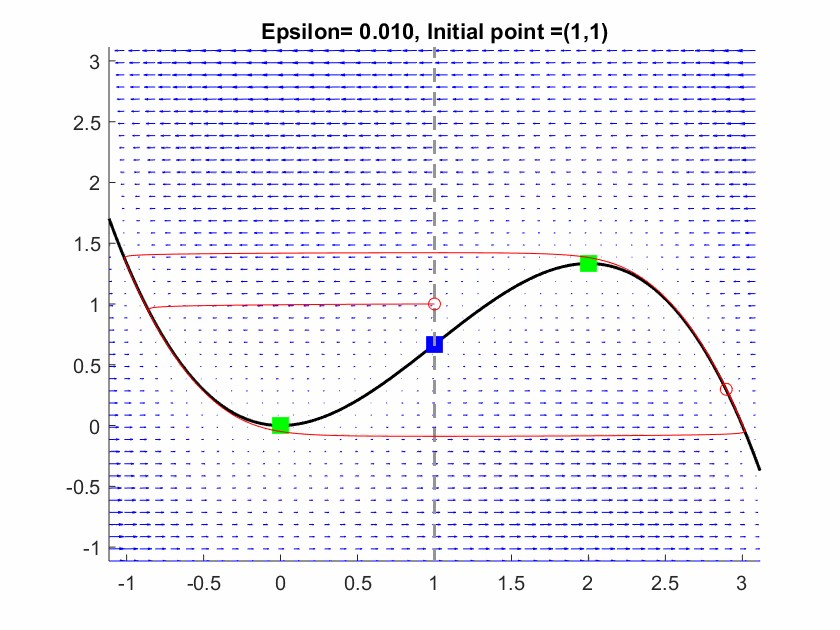
\includegraphics[width=.8\linewidth]{vdPe001-Moment-normal}
			\caption{The flow on the \vdp for a small $ \epsilon $.} \label{fig: vdp normal}
		\end{subfigure}
		\hfill
		\begin{subfigure}[t]{0.45\textwidth}
			\centering
			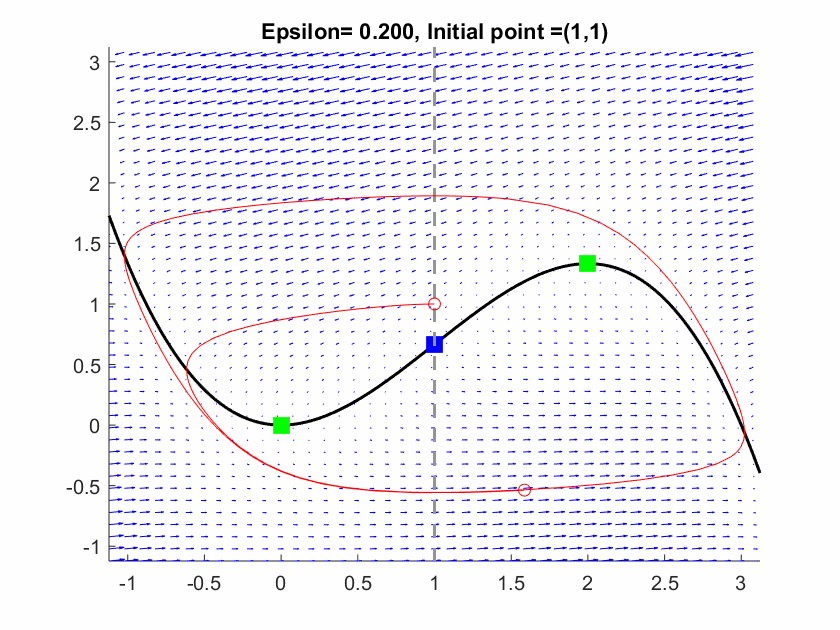
\includegraphics[width=.8\linewidth]{vdPe02-Moment-big-e}
			\caption{The flow on the \vdp for a larger $ \epsilon $.} \label{fig: vdp e.2}
		\end{subfigure}
		
%		\vspace{1cm}
%		\begin{subfigure}[t]{0.45\textwidth}
%			\centering
%			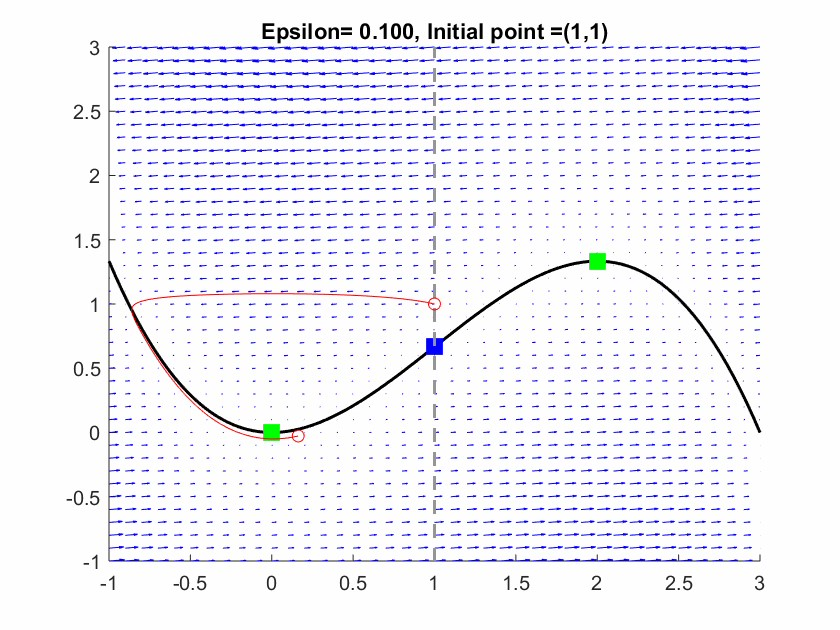
\includegraphics[width=.8\linewidth]{vdPhopf-Moment-3.jpg}
%			\caption{The flow as it intersects with the fold point.} \label{fig:timing3}
%		\end{subfigure}
%		\hfill
%		\begin{subfigure}[t]{0.45\textwidth}\centering
%			% just an empty subfigure to shift C below A
%			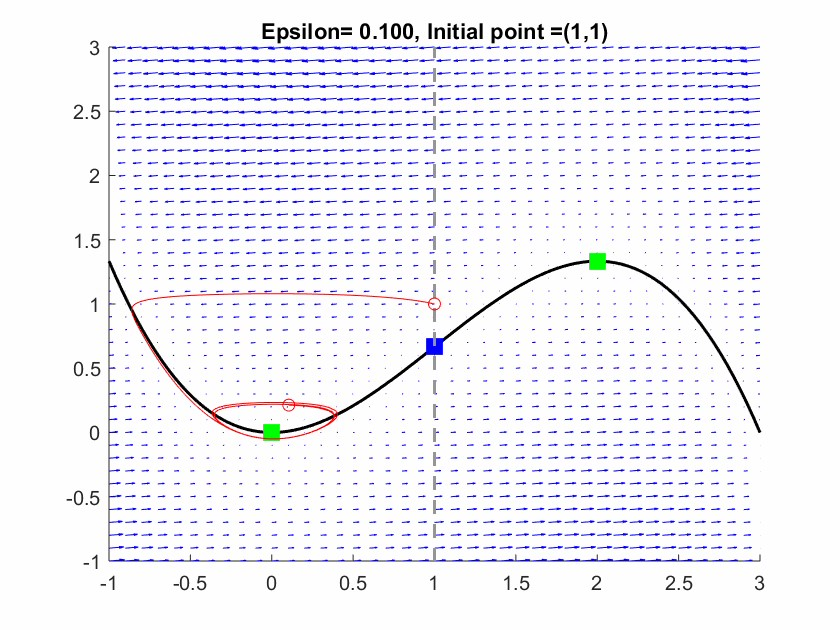
\includegraphics[width=.8\linewidth]{vdPhopf-Moment-4.jpg}
%			\caption{The Hopf bifurcation due to the canard point.}\label{fig:timing4}
%		\end{subfigure}
	\caption{Flow on the \vdp system.}
	\label{fig: vdp flow diagram e}
\end{figure}
++++ weave out +++++++++



























\section{Canard Points}
\begin{figure}[h!]
	\centering
	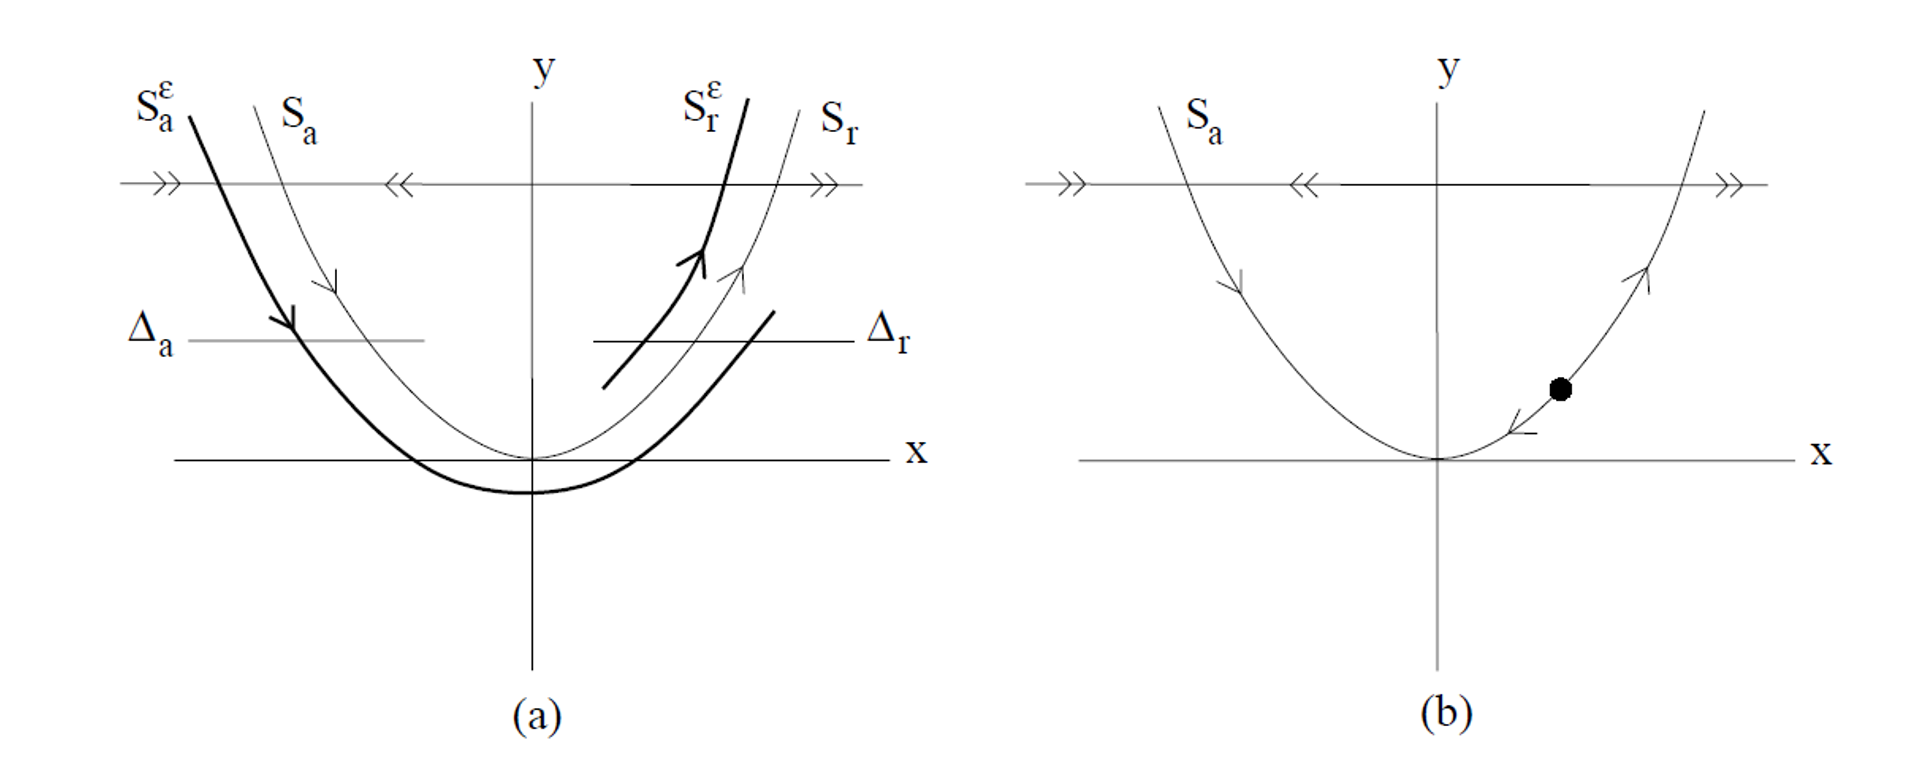
\includegraphics[height=5cm,width=8cm]{Canard_Point.png}
	\caption{The reduced flow where a) $\lambda=0$ and b) $\lambda>0$.}
	\label{fig: Canard Point}
\end{figure}\newpage



Considering the Van der Pol System as before:
\begin{equation}
\begin{aligned}
&x'=-y+x^2-\dfrac{x^3}{3},\\
&y'=\epsilon(x-1),\\
\end{aligned}
\tag{\ref{eq: Fast System}}
\end{equation}
we notice that the equilibrium of the system depends on the two nullclines $ x'=0$ and $y'=0$. These are in the shape of a cubic funcion and in the shape of a vertical line at $x=1$. 
The idea in this section is to replace the nullcline $x=1$ by $x = \lambda$. This can be seen as shifting the equilibrium of the system along the critical manifold $S$ by varying the parameter $\lambda$.
This gives rise to a generalised Van der Pol system:
\begin{equation}
\begin{aligned}
&x'=-y+x^2-\dfrac{x^3}{3},\\
&y'=\epsilon(x-\lambda).\\
\end{aligned}
\label{eq: canard system}
\end{equation}
In this section, the dynamics in system \ref{eq: canard system} is analysed. In order to do so, we need the definition of a canard.
\begin{definition}{\textbf{ Canard}}[\citealp{Kuehn}]
A trajectory of a fast-slow system is called a canard if it stays within $O(\epsilon)$ close to the repelling branch $S^r$ of the slow manifold $S$, for some time of $O(1)$ on the slow time scale $\tau = \epsilon t$.
\end{definition}
Furthermore, the following definition turns out to be useful as well:
\begin{definition}{\textbf{Maximal Canard}}[\citealp{Kuehn}] \label{maxcanard}
The trajectory passing through the intersection of $S^a$ and $S^r$ is called a maximal canard. 
\end{definition}
\begin{definition}{\textbf{Singular Canard}}
\end{definition}
The intuition of the canard problem close to a fold point is given in Figure \ref{fig: Canard Point}.
Equivalently to the analysis of the fold point in Section \ref{sec:the-van-der-pol-equation}, some nondegeneracy conditions are defined. These are, as before, applied at the fold point $(0,0)$. Note that in contrast to the nondegeneracy conditions in (\ref{NonDeg}), the transversality condition $g(0,0,0) \neq 0$ is not satisfied. Therefore higher order conditions on $g$ have to be employed, in particular these are nonzero derivatives of $g$ with respect to $x$ and $\lambda$. The fact that $g_x(0,0,0) \neq 0$ guarantees the existence of transversal intersection of the two nullclines, which is crucial in order to conclude persistence of the dynamics later on \citep{kuehn}. 
The nondegeneracy and transversality conditions for the canard case are  \citep{krupa2001},
\begin{equation}
f(0,0,0,0)=0, \ \pd{}{x}f(0,0,0,0)=0, \ g(0,0,0,0)=0, \label{eq: canard sing condition}
\end{equation}
\begin{equation}
\begin{aligned}
&\pd{^2}{x^2}f(0,0,0,0)\neq 0, \ \pd{}{y}f(0,0,0,0)\neq 0,\\
&\pd{}{x}g(0,0,0,0)\neq 0, \ \pd{}{\lambda}g(0,0,0,0)\neq 0. \label{eq: canard non-d condition}
\end{aligned}
\end{equation}
Now that these conditions have been defined we can consider, equivalent to the argument in Section \ref{sec: extended sys blowup}, the extended \vdp system,
\begin{equation}
\begin{aligned}
&x'=-y+x^2-\dfrac{x^3}{3},\\
&y'=\epsilon(x-\lambda),\\
&\epsilon'=0,\\
&\lambda'=0,\\
\end{aligned}
\label{eq: canard system}
\end{equation}
where the change in $\epsilon$ and $\lambda$ are constant. 
Now, for the remainder of the section, we apply the method of \citet{krupa2001} to the Van der Pol System. The canonical form for the Canard System is:
\begin{equation} \label{canardysy2var}
	\begin{aligned}
		x'&=-yh_1(x,y,\epsilon,\lambda)+x^2h_2(x,y,\epsilon,\lambda) + \epsilon h_3(x,y,\lambda,\epsilon)\\
                        &= -y + x^2 \left( 1- \frac{x}{3} \right),\\
		y'&=\epsilon(xh_4(x,y,\epsilon,\lambda)-\lambda h_5(x,y,\epsilon,\lambda) + y h_6(x,y,\lambda,\epsilon)) \\
                        &= \epsilon( x- \lambda).
	\end{aligned}
\end{equation}
It follows that $h_1 = 1$, $h_2 = 1-\frac{x}{3}$, $h_3=0$, $h_4 =1$, $h_5=1$ and $h_6=0$.
It is possible to find a $\lambda>0$, for which an equilibrium on the repelling branch $S_r$ exists for the reduced dynamics.
The following definition can be made in order to simplify the following computations:

\begin{align*}
a_1=\pd{}{x}h_3(0,0,0,0)=& 0 \ \ \
a_2=\pd{}{x}h_1(0,0,0,0)= 0\ \ \ 
a_3=\pd{}{x}h_2(0,0,0,0)=-\frac{1}{3}\\
a_4&=\pd{}{x}h_4(0,0,0,0)=0\ \ \
a_5=h_6(0,0,0,0)=0.
\end{align*}
Furthermore, we can define the quantity:
\begin{align*}
A=-a_2+3a_3-(2a_4+2a_5)=-1,
\end{align*}
which is important in the following analysis, in particular for $A \neq 0$ \citep{krupa2001}. 
Similar to the procedure in Section \ref{sec: VDP Blowup}, sections of the dynamical system can be defined, in order to monitor the in- and outgoing trajectories. In this case we are interested in two sections of the neighbourhood $U$, defined as in Section \ref{sec: VDP Blowup}, that monitor $S^a$ and $S^r$ close to the fold point.
Let $ \Delta_a = \{ (x,\rho^2), x \in  I_a \}$ and $\Delta_r= \{ (x,\rho^2), x \in  I_r \}$, where $I_a,I_r$ are intervals on the real line and $\rho$ is sufficiently small.
Futhermore, define $q_a$ to be the point on $\Delta_a$ that belongs to the attracting branch $S^a$, while $q_r$ is equivalently defined as the point on $\Delta_r$ that corresponds to $S^r$. Finally, we are in the position to define the transition map $\pi: \Delta^a \to \Delta^r$, compare to Section \ref{sec: VDP Blowup}.
Following this, \citet{krupa2001} discuss the existence of a critical value for $\lambda$ (denoted $\lambda_c$), where the two branches $S_r$ and $S_a$ must connect in a smooth fashion.  
The transition map $\pi$ has to map the point $q_a$ to $q_r$, if the branches are connected, and the trajectory passing through the fold point is called the maximal canard, see Definition \ref{maxcanard}
The following theorem describes the technical details involved, and some of the results are derived by the following analysis.
\begin{theorem}[\cite{krupa2001}]
	Assume that system (3.1) satisfies the defining non-degeneracy conditions (Equations \ref{eq: canard sing condition} and \ref{eq: canard non-d condition}) of a canard point. Assume that the solution $ x_0(t) $ of the reduced problem connects $ S_a $ to $ S_r $. Then there exists $ \epsilon_0 > 0 $ and a smooth function $\lambda_c(\sqrt{\epsilon})$ defined on $ [0, \epsilon_0] $ such that for $\epsilon \in (0, \epsilon_0)$ the following assertions hold:
	\begin{itemize}
		\item $ \pi(q_{a,\epsilon})=q_{r,\epsilon} $ iff $ \lambda=\lambda_c(\sqrt{\epsilon}) $.\\
		\item The function $ \lambda_c $ has the expansion
		 \begin{equation*}
			\lambda_c(\sqrt{\epsilon})=-\epsilon(\frac{a_1+a_5}{2}+\frac{A}{8})+O(\epsilon^\frac{3}{2}).
			\end{equation*}
			\item The transition map $\pi$ is defined only for $\lambda$ in an interval around $ \lambda_c(\sqrt{\epsilon}) $ of width $ O(\exp(-\frac{c}{\epsilon})) $ fo some $ c>0 $.
			$$ \pd{}{\lambda}(\pi(q_{a,\epsilon})-q_{r,\epsilon})|_{\lambda=\lambda_c(\sqrt{\epsilon})}>0  $$
		
	\end{itemize}
\label{Theorem 3.1}
\end{theorem}
%Consider Canard cycles and center manifolds / Freddy Dumortier, Robert Roussarie. for more details on canards in \vdp. ++++++Kieran, what do you mean here+++++
%



\subsection{Canard Blow-up}
Now similarly to Section \ref{sec: VDP Blowup}, we consider a transformations of the coordinate system in order to analyse the dynamics in the neighbourhood of the non-hyperbolic equilibrium induced by the canard point. %(++++++ is the eq. induced by lambda??++++).
 The transformations are taken from \citep{krupa2001} and are,
\begin{equation}
x=\bar{r}\bar{x}, \ y=\bar{r}^2y, \ \epsilon=\bar{r}^2\bar{\epsilon}, \ \lambda=\bar{r}\bar{\lambda}.
\end{equation}
Now that we have established these transformation, the charts $K_1$ and $K_2$ can be introduced,  but it is not necessary to consider the third chart, $K_3$. Since the attracting slow manifold connects to the repelling slow manifold, the flow will `bend back' from $K_2$ into $K_1$ instead of leaving the neighbourhood $U$ in the direction of the fast flow, which was described by $K_3$ in Section \ref{sec: VDP Blowup}. 
This pheonomenon can be observed in Figure \ref{fig: flow in canard}, where the trajectory stays close to $S^r$ after passing the fold point.
\begin{figure}[h!]
	\centering
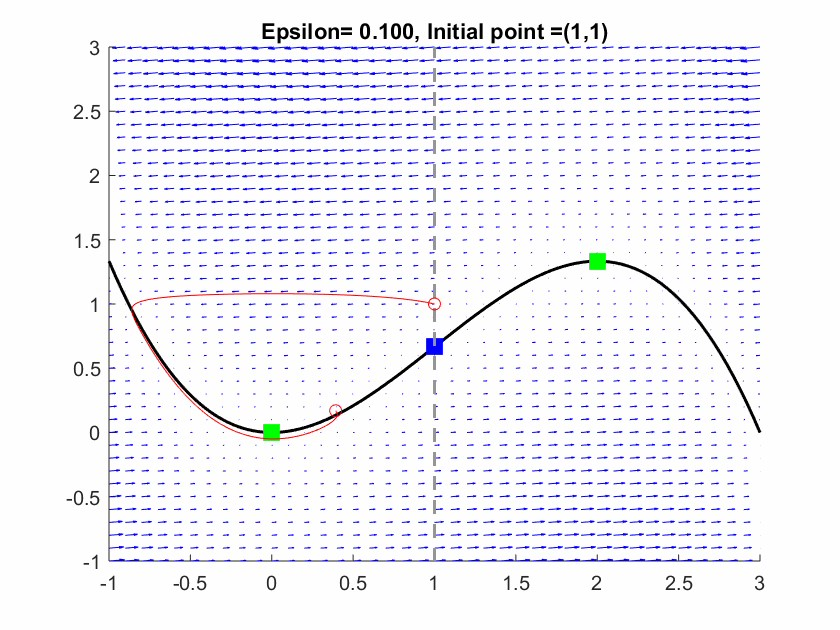
\includegraphics[width=8cm, height=6cm]{Images/vdPhopf-Moment-bendback}
	\caption{The \vdp system for the canard case.}
	\label{fig: flow in canard}
\end{figure}\newpage
Again, equivalently to the procedure in Section \ref{sec: VDP Blowup}, we can define the coordinate transformation for the charts. Note, that in contrast to the generic Blow-Up in Section \ref{sec: VDP Blowup}, the coordinate system is now in $\mathbf{R}^4$, and not in $\mathbf{R}^3$. In chart $K_1$, $y_1=1$, while in $K_2$, $\epsilon_1=1$ and then:
\begin{subequations}
	\begin{align}
	&x=r_1x_1, \ y=r_1^2, \ \epsilon=r_1^2\epsilon_1, \ \lambda=r_1\lambda_1 \label{eq: coordiante K1}\\ 
	&x=r_2x_2, \ y=r_2^2y_2, \ \epsilon=r^2_2, \ \lambda=r_2\lambda_2 \label{eq: coordinate K2}.
	\end{align}
\end{subequations}
Furthermore, we can define the coordinate change between the two charts as follows:
\begin{lemma}
Let $\kappa_{12}$ denote the change of coordinates from $K_1$ to $K_2$. Then $\kappa_{12}$ is given by
\begin{align*}
x_2 = x_1 \epsilon_1^{-1/2}, \ \ \ y_2 = \epsilon_1^{-1}, \ \ \ r_2 = r_1 \epsilon_1^{1/2}, \ \ \ \lambda_2 = \epsilon_1^{-1/2} \lambda_1,
\end{align*}
for $\epsilon_1 >0$.
Similarly $\kappa_{21}=\kappa_{12}^{-1}$ is given by
\begin{align*}
x_1 = x_2 y_2 ^{-1/2}, \ \ \ r_1 = r_2 y_2 ^{1/2}, \ \ \ \epsilon_1 = y_2^{-1}, \ \ \ \lambda_1 = \lambda_2 y_2^{-1/2},
\end{align*}
for $y_2 >0$.
\end{lemma}

We are now in the position to begin with the analysis in the charts, and will first consider chart $K_2$, since, as in Section \ref{sec: VDP Blowup}, $K_2$ holds the most information. 

\subsubsection{Dynamics in \texorpdfstring{$K_2$}{K2}}
%<<<<<<< HEAD
We start by noting that we are considering our invariant plane at $r_2=0$ which will significantly simplify our system for $K_2$. Further we should note that we are taking a transformation in time, $\od{r}{t_2}=\od{t}{t_2}\od{r}{t}=\frac{1}{r_2}\od{r_2}{t}$, as well as in our coordinates. Then if we substitute our time transformation and Equation  \ref{eq: coordinate K2} into our system of Equations \ref{eq: canard system} we find, 
\begin{subequations}
	\begin{align}
	r_2^2x_2' - r_2x_2r_2'&=-r_2^2y_2h_1+r^2_2x^2_2h_2,\notag\\
	\implies x'_2&=-y_2+x_2^2-r_2G_2(x_2,y_2), \label{eq k2 x trans}\\
	%     \end{aligned}
	% \end{equation*}
	% \begin{equation}
	%     \begin{aligned}
	r^3_2y_2'-3r_2^2y_2r_2'&=r^2_2(r_2x_2h_4-r_2\lambda_2h_5),\notag\\
	\implies y_2'&=x_2-\lambda_2+r_2G_2(x_2,y_2), \label{eq: K2 y trans}
	\end{align}
	\label{eq: reduced canard k2}
\end{subequations}
\noindent where we note that $h_j=h_j(x,y,\epsilon,\lambda)$ for $j=1,2,3,4,5$.  Notice that we have included an additional term in Equation \ref{eq: reduced canard k2} - we define $G_2(x_2,y_2)$ in the following way, $G(x_2,y_2)=(G_1(x_1,y_1),G_2(x_2,y_2))^T=(-\frac{x^3_2}{3},0)^T$. The reason we also define this vector is to aide in the Melnikov computations which we will see later. Then combing this yields our complete system
\begin{subequations}
	\begin{align}
	x'_2&=-y_2+x_2^2-r_2G_1(x_2,y_2) =-y_2+x_2^2-r_2\left(-\frac{x^3_2}{3} \right) ,\tag{\ref{eq k2 x trans}}\\
	y_2'&=x_2-\lambda_2+r_2G_2(x_2,y_2)= x_2-\lambda_2, %\label{eq: K2 y trans}
	\tag{\ref{eq: K2 y trans}}
	\end{align}
\end{subequations}
recalling that $r_2'=\lambda_2'=0$. Moreover, \citet{krupa2001} discusses that for this chart we have an interesting result. They note that at $r_2=\lambda_2=0$ our system is integrable which allows us to define a constant of motion $H(x_2,y_2)=\frac{1}{2}\exp{(-2y_2)}\left(y_2-x^2_2+\frac{1}{2}\right)$. For clarity we will first proceed with deriving this equation of motion. Firstly, multiply each equations by, $e^{2y_2}e^{-2y _2}=1$, and define sections of each equation as partial derivatives of $H$ \st, 
\begin{align}
x_2' &=e^{2y_2}e^{-2y_2}( -y_2 +x_2^2 ) =e^{2y_2}\pd{H}{y_2}(x_2,y_2) \\
y_2' &= - e^{2y_2}e^{-2y_2}(-  x_2)=-e^{2y_2}\pd{H}{x_2}(x_2,y_2).
\end{align}
Then we integrate $ \pd{H}{x_2}(x_2,y_2) = -e^{-2y_2} x_2  $ to give,
\begin{align*}
%&\Rightarrow H(x_2,y_2) = \int -e^{-2y_2} x_2 dx\\
 H(x_2,y_2) = - \frac{1}{2} x^2 e^{-2y_2} + C(y),
\end{align*}
where $C(y)$ is the constant of integration, which depends on $y$.
Then, by taking the derivative with respect to $y$ and setting it equal to the expression $\pd{H}{y_2}(x_2,y_2)=e^{-2y_2}( -y_2 +x_2^2 )$, we can find the value for $C(y)$ as follows: 
\begin{align*}
\pd{H}{y_2}(x_2,y_2)&= x^2 e^{-2y_2} + C'(y)\\
%&= e^{-2y_2}( -y_2 +x_2^2 )\\
\Rightarrow C'(y) &= - y_2 e^{-2y_2}
\end{align*}
Finally we integrate $C'(y)$ in order to find an explicit expression for $H$,
\begin{align*}
C(y) = \int - y_2 e^{-2y_2} dy = \frac{1}{2} y_2 e^{-2y_2} + \frac{1}{2} e^{-2y_2} + const,
\end{align*}
using integration by parts.
Then, the final expression is:
\begin{align}
H(x_2,y_2)&=- \frac{1}{2} x^2 e^{-2y_2} + \frac{1}{2} y_2 e^{-2y_2} + \frac{1}{2} e^{-2y_2} + c\\
&= \frac{1}{2}e^{-2y_2}\left(y_2-x^2_2+\frac{1}{2}\right) +c. \label{eq: const of motion}
\end{align}
Note that without loss of generality we can choose $c=0$ because we are interested in the level curves of $H$ and $H=h$. Now that we have shown how the constant of motion is constructed we will consider our reduced system, that we have an equilibrium at the origin, implying that $H(x_2,y_2)=h$. Considering the reduced system (Equation \ref{eq: reduced canard k2}) we have from $ H(x_2,y_2)=0 $ that,
\begin{subequations}
	\begin{align}
	x_2'&=\frac{1}{2}\ \	\implies x_2=\frac{t_2}{2}+A, \label{canard: trajectory x}\\
	y_2'&=\frac{t_2}{2}\ \implies y_2=\frac{t_2^2}{4}-\frac{1}{2}, \label{canard: trajectory y}
	\end{align}
\end{subequations} 
where we have directly integrated Equation \ref{canard: trajectory x} with respect to our time ($ t_2 $). However, we note that we are able to choose $ A=0 $, as we are considering an autonomous (time-invariant) system. Then for Equation \ref{canard: trajectory y} we are able to rearrange the constant of motion at zero to give, $ y_2=x_2^2-\frac{1}{2} $. Clearly from this analysis we are then able to define our trajectories in terms of $ \gamma_{c,2} $, 
\begin{equation}
\gamma_{c,2}(t_2)=(x_{c,2}(t_2),y_{c,2}(t_2))=\left(\frac{t_2}{2},\frac{t^2_2}{4}-\frac{1}{2}\right).   \label{eq: gamma c2}
\end{equation}
Now that we have established that we must have a flow on our second chart, then there must also exist transition maps. Therefore this now enables us to consider the first chart in the following section.


\subsubsection{Dynamics in \texorpdfstring{$K_1$}{K1}}\label{sec:dynamics-in-texorpdfstringk1k1}
For $K_1$ we follow a similar approach to the above. We will use the transformations, 
\begin{equation}
x=r_1x_1, \ y=r_1^2, \ \epsilon=r_1^2\epsilon_1, \ \lambda=r_1\lambda_1 \tag{\ref{eq: coordiante K1}},
\end{equation}
to find the relevant pathways of our flows. Now if we first consider the $r_1$ component, 
\begin{align}
2r_1^2r_1'=r_1^2\epsilon(r_1x_1-r_1\lambda_1), \label{canard: r1}
\end{align}
where we define $F=F(x,y,\epsilon,\lambda)=x_1-\lambda_1+O(r_1(r_1+\lambda_1)$. Next we consider $x=r_1x_1$,
\begin{align*}
r_1r_1'x_1+r_1^2x_1'&=-r_1^2+r_1^2x_1^2,\\
x_1'&=-1+x_1^2-\frac{x_1r_1'}{r_1},
\end{align*}
where we can use Equation \ref{canard: r1} to simplify this further,
\begin{align}
x_1'=-1+x_1^2-\frac{x_1}{r_1}\left(\frac{r_1\epsilon_1F}{2}\right). \label{eq: canard x1}
\end{align}
We now consider $\epsilon=\epsilon_1r_1^2$ and noting $\epsilon'=0$. Then we have, $r_1^3\epsilon'=-2r_1^2\epsilon_1r_1'$, where we can use Equation \ref{canard: r1} to simplify to,
\begin{align}
\epsilon'=-\epsilon_1^2F. \label{canard: epsilon k1}
\end{align}
Our last transformation is for our new coordinate $\lambda=r_1\lambda$, noting that $\lambda'=0$. Similarly to the above we find $r_1^2\lambda_1'+r_1\lambda_1r_1'=0$ then, 
\begin{equation}
\lambda'_1=-\frac{\lambda_1\epsilon_1F}{2}, 
\end{equation}
which is a trivial rearrangement as seen in Equation \ref{canard: epsilon k1}. Now if we combine the above we find that our transformed system is of the following form,
\begin{subequations}
	\begin{align}
	r_1'&=\frac{\epsilon}{2}(r_1x_1-r_1\lambda_1), \\
	% \label{canard: r1}
	x_1'&=-1+x_1^2-\frac{x_1\epsilon_1F}{2},\\
	\epsilon'&=-\epsilon_1^2F,\\
	\lambda'_1&=-\frac{\lambda_1\epsilon_1F}{2}.
	\end{align}
	\label{canard: system of equations}
\end{subequations}
From this system we are now able to make some deductions. We first can observe that the hyperplanes are along the $r_1=\epsilon_1=\lambda_1=0$ with an invariant line at $l_1=\{(x_1,0,0,0): x_1\in\mathbb{R}\}$ \citep{krupa2001}. As \citet{krupa2001} discusses the equilibria present at the end of both of our branches - Figure \ref{fig: Canard Point} - which are found at $p_a=(-1,0,0,0) \ \text{and} \ p_r=(1,0,0,0)$ \citep{krupa2001}. Now we can go one step further, we can consider Equation \ref{canard: system of equations} and find the eigenvalues of the system for the invariant planes. We find that, 
\begin{equation}
J-\sigma I= \begin{bmatrix}
2x-\sigma & 0 & 0 & 0  \\
0 & -\sigma & 0 & 0&\\
0 & 0 & -\sigma & 0 \\
0 & 0 & 0 & -\sigma
\end{bmatrix},
\end{equation}
which clearly has three zero eigenvalues and one non-zero eigenvalue $\sigma=\pm 2$. Which further empahsises that our equilibrium point is non-hyperbolic. As a result we intuitively expect that something interesting occurs at this point. In the section following we will be considering what effect these mappings and eigenvalues will have on our system.


\subsection{Effect of the Canard Point}\label{sec:effect-of-the-canard-point}
Now that we have shown that there must exist a flow around our fold point we should now consider the global effect of the canard point. We can see by considering the  system of Equations \ref{canard: system of equations} that our equilibriums are at $ (x,y)=(\lambda,\lambda^2[\frac{1-\lambda}{3}]) $ and find the eigenvalues from the matrix, 
\begin{equation}
A-\sigma I=\begin{bmatrix}
2x-x^2-\sigma&-1&0&0\\
\epsilon&-\sigma&x-\lambda&-\epsilon\\
0&0&-\sigma&0\\
0&0&0&-\sigma
\end{bmatrix}=\sigma^2(\sigma^2+\sigma(x^2-2x)+\epsilon).
\end{equation}
%\begin{equation}
%A-\sigma I=\begin{bmatrix}
%2\lambda-\lambda^2-\sigma&-1&0&0\\
%\epsilon&-\sigma&0&-\epsilon\\
%0&0&-\sigma&0\\
%0&0&0&-\sigma
%\end{bmatrix}.
%\end{equation}
%\textbf{Then our eigenvalues are, $ \sigma=(2-x)x \ \text{and} \ \sigma=0 $, noting that we have an upper triangular matrix. Then we can note that we have a complex eignevalue which causes a Hopf bifurcation, as shown below:}%wrong maths
From this we are about to find the eigenvalues of the system, $ \sigma=0 $ and $ \sigma=\frac{2x-x^2\pm\sqrt{(x^2-2x)^2-4\epsilon}}{2} $. Then we consider the values at our equilibrium, $ x=\lambda $, to find that we have a Hopf Bifurcation when $ 4\epsilon>(x^2-2x)^2 $ or when $ \lambda=2 \ \text{or} \ 0 $. This then leads to the following trajectories within the flow - Figure \ref{fig: 4 canard }.

\begin{figure}[h!]
	\centering
	\begin{subfigure}[t]{0.45\textwidth}
		\centering
		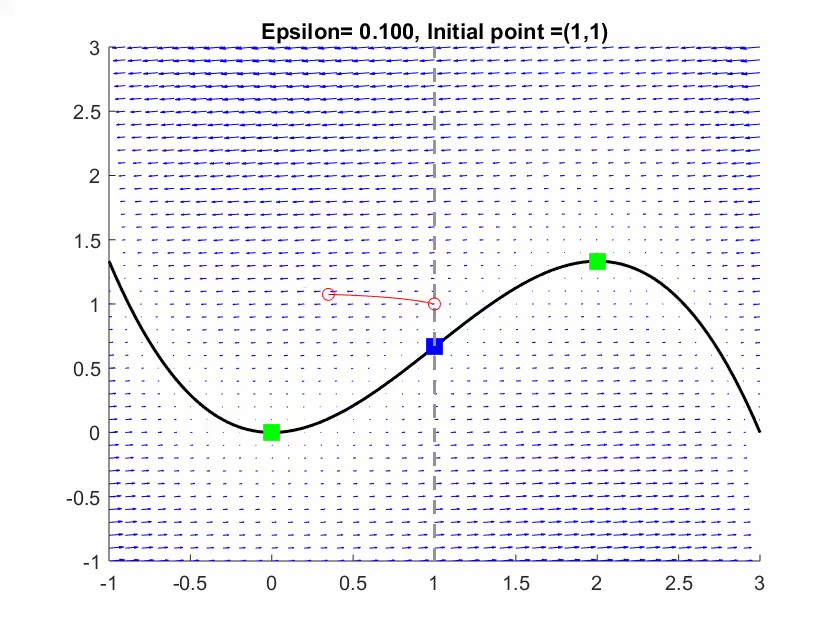
\includegraphics[width=.8\linewidth]{vdPhopf-Moment-1.jpg}
		\caption{The initial flow within the system.} \label{fig:timing1}
	\end{subfigure}
	\hfill
	\begin{subfigure}[t]{0.45\textwidth}
		\centering
		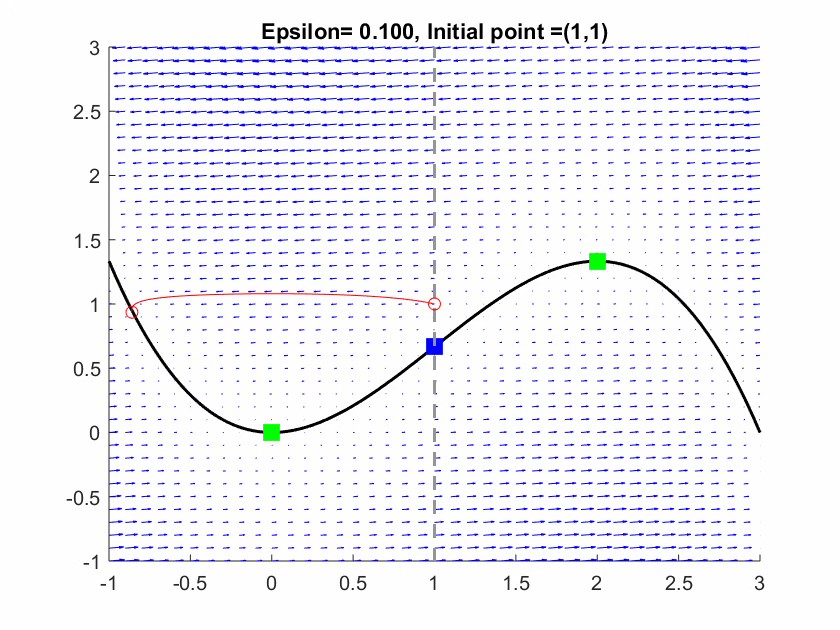
\includegraphics[width=.8\linewidth]{vdPhopf-Moment-2.jpg}
		\caption{The flow as it hits the slow manifold.} \label{fig:timing2}
	\end{subfigure}
	
	\vspace{1cm}
	\begin{subfigure}[t]{0.45\textwidth}
		\centering
		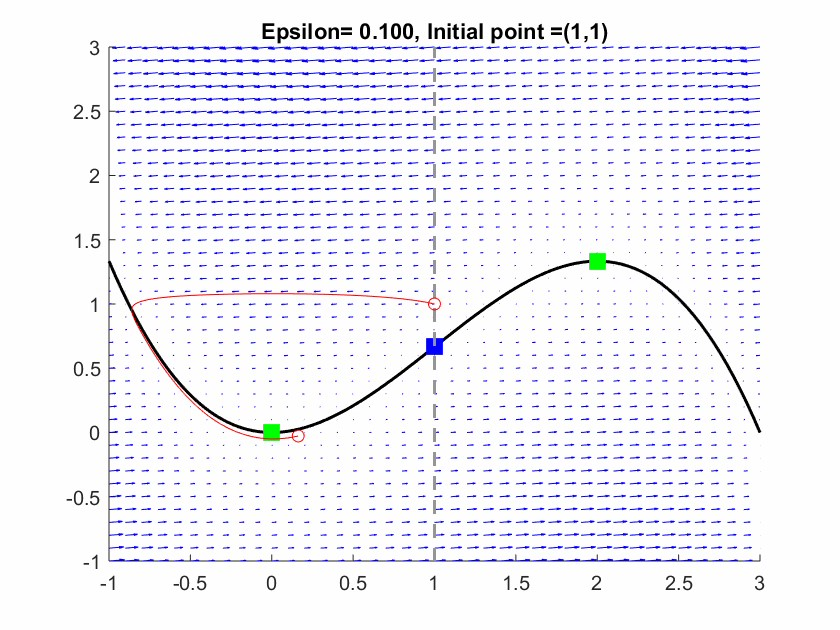
\includegraphics[width=.8\linewidth]{vdPhopf-Moment-3.jpg}
		\caption{The flow as it intersects with the fold point.} \label{fig:timing3}
	\end{subfigure}
	\hfill
	\begin{subfigure}[t]{0.45\textwidth}\centering
		% just an empty subfigure to shift C below A
		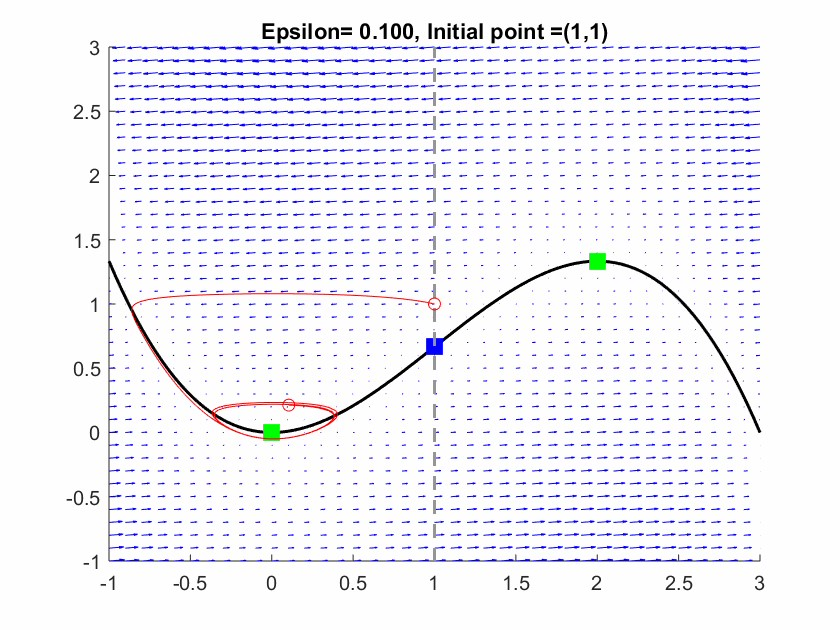
\includegraphics[width=.8\linewidth]{vdPhopf-Moment-4.jpg}
		\caption{The Hopf bifurcation due to the canard point.}\label{fig:timing4}
	\end{subfigure}\vspace{1cm}
	\begin{subfigure}[t]{0.45\textwidth}\centering
		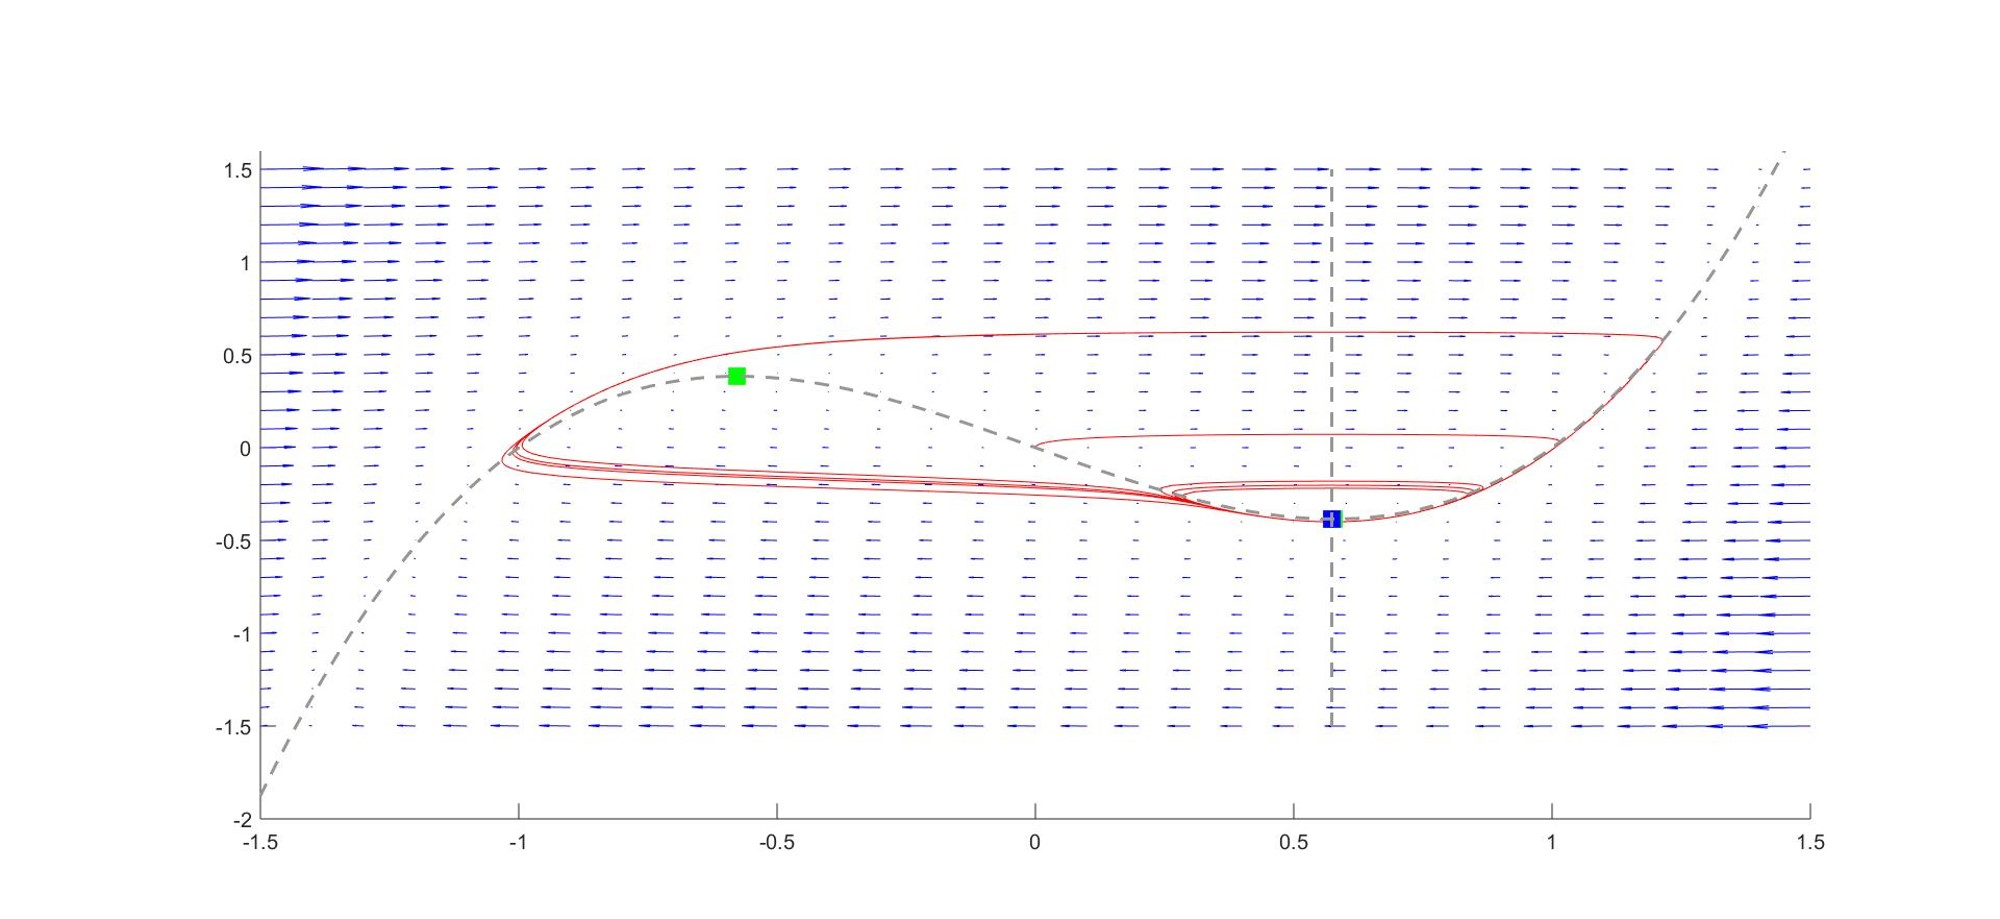
\includegraphics[width=.8\linewidth, height=6cm]{Code/behaviourswitch-pres}
		\caption{Growth of the Hopf bifrucation leading to the formation of a Canard explosion.}
		\label{fig: hopf growth}
	\end{subfigure}
	\caption{The trajectories associated with the canards case of the \vdp system.}
	\label{fig: 4 canard }
\end{figure}\newpage
From Figure \ref{fig: 4 canard } we can see the progression of our flow over the system. From Figure \ref{fig:timing1} we see that the flow starts at an initial condition of $ (x,y)=(1,1) $ and travels along the fast flow towards the attracting branch. Then from Figure \ref{fig:timing2} the flow has hit the attracting branch, where it then follows along the slow flow towards the fold point at $ (x,y)=(0,0) $, which is described by Figure \ref{fig:timing3}. Then from Figures \ref{fig:timing3} and \ref{fig:timing4} we can observe the Hopf bifurcation. This is because we make note that the canard point is present at $ -\lambda $, which in essence pushes the flow up the repelling branch (see Figure \ref{fig: Canard Point}) until the flow is sufficiently far from the fold point where it will then repel towards the attracting branch, starting the growing oscillations - Figure \ref{fig:timing4}. When the Hopf bifurcation is large we would then expect to see a jump in our solution to an attracting branch - Figure \ref{fig: hopf growth}.

%\begin{figure}[h!]\centering
%	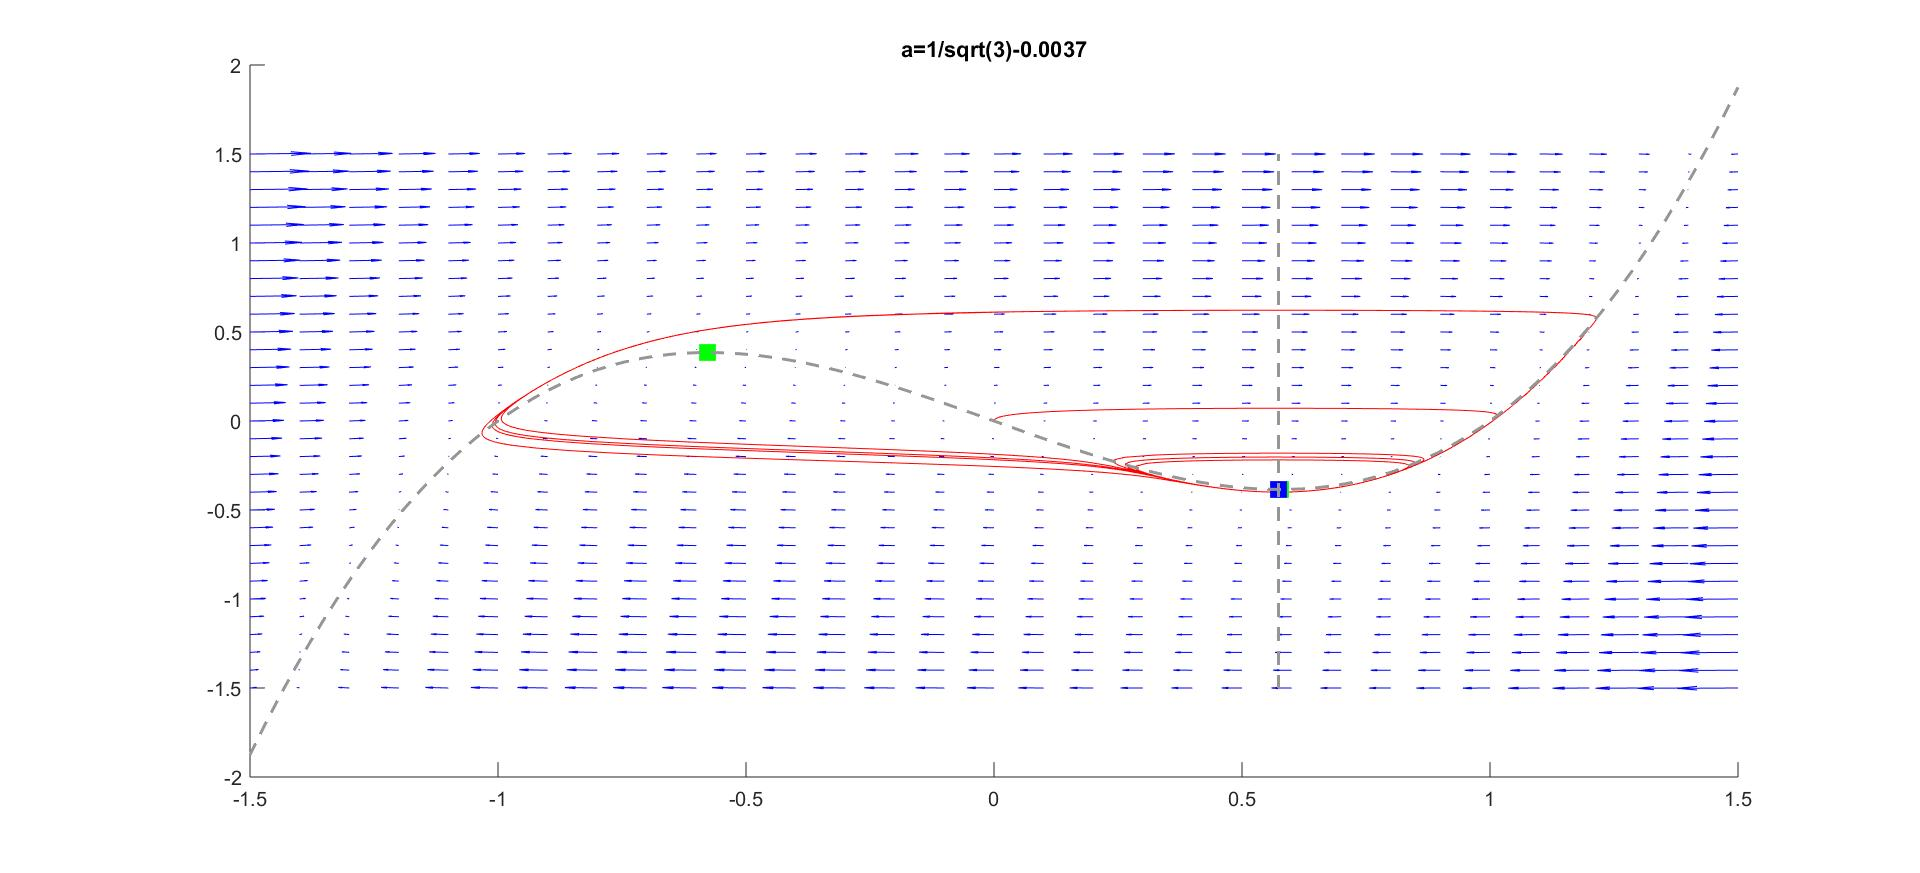
\includegraphics[height=8cm,width=6cm]{Code/behaviourswitch}
%	\caption{Growth of the Hopf bifrucation leading to the formation of a Canard explosion.}
%	\label{fig: hopf growth}
%\end{figure}\newpage
%
%Moreover, it is worth noting that our Hopf bifurcation only exists when we are in an arbitrarily small region, $ O(\epsilon) $, due to the local nature of the theorem \cite{Eckhaus}. 
%\begin{figure}[h!]\centering
%%	\includegraphics[]{}
%	\caption{Development of the Hopf Bifurcation. \textbf{Tom can you screenshot the flow in 4 places?}}
%	\label{fig: Hopf}
%\end{figure}
%Figure \ref{fig: 4 canard } shows that we have an unstable periodic solution within our canard system. In addition to this we know that our canard system will only exist within a small region of $ O(\epsilon) $ \citep{Eckhaus}. Moreover, we can see from Figure \ref{fig: Hopf} that our flow follows the expected path, as we saw in ++++++++++++++++++++++++\\
%%%%%%%%%%%%%%%%%%%%%%%%%%%%%%%%%%%%%%%%%%%%%%%%%%%%%%%%%%%%%%%%%%%%%%%%%%%%%%%%%%%%%%%%%%%%%%%%%%%%%%%%%%%%%%%%%%%%%%%%%%%%%%%%%%%%%%%%%%%%%%%%%%%%%%%%%%%%%%%%%%%%%%%%%%%%%%
%\subsubsection{Singular Hopf Bifurcation}\label{sec:singular-hopf-bifurcation}
%Furthermore, in the \vdp we are able to find a singular Hopf Bifurcation when $ \lambda=1 $. Then to model this behaviour we need to consider a small perturbation along the slow flow where we will have, from Equation \ref{eq: canard system},%discuss what the solutions for x is in the paper 
%\begin{equation}
%\dot{y}=\lambda-x+\bar{\nu} y,
%\end{equation}
%where $ \nu $ is of order $ O(\epsilon) $, thus small. We can immediately see that when $ \bar{\nu}=0 $ that we have our original flow at our equilibrium but we are now able to perturb our flow over a small domain, which are described in Figures \ref{fig: Hopf}. We can also see how our system behaves when our $ \nu $ is of larger order than $ O(\epsilon) $,
%
%\begin{figure}[h]\centering
%	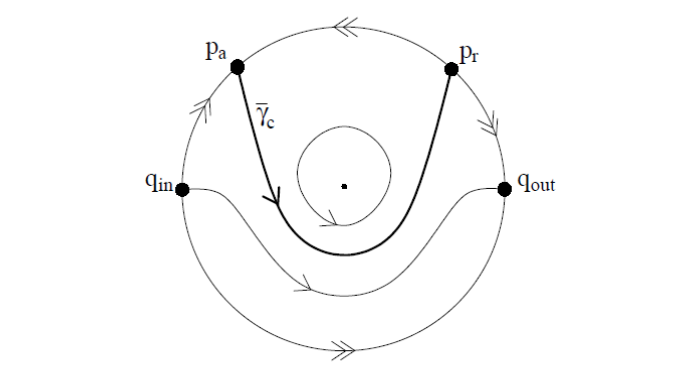
\includegraphics[height=6cm,width=10cm]{Images/CanardPointcircle}
%	\caption{The flow within our canard system \citep{krupa2001}.}
%	\label{fig: canard flow circle}
%\end{figure}\newpage
%where it is clear that our Hopf bifurcation is the periodic solution in the centre of Figure \ref{fig: canard flow circle} but we can see that below our special flow $ \bar{\gamma_c} $ (for the flow outside of the domain $ O(\epsilon) $),our solution traverses through our equilbrium into our fast flow as we would expect in our original system.

%%%%%%%%%%%%%%%%%%%%%%%%%%%%%%%%%%%%%%%%%%%%%%%%%%%%%%%%%%%%%%%%%%%%%%%%%%%%%%%%%%%%%%%%%%%%%%%%%%%%%%%%%%%%%%%%%%%%%%%%%%%%%%%%%%%%%%%%%%%%%%%%%%%%%%%%%%%%%%%%%%%%%%%%%%%%%%

%\subsubsection{Singular Hopf Bifurcation}\textbf{Does this section tie in anywhere else?}
%In this section we will further expand on our Hopf Bifurcation of the previous section (Section \ref{sec:effect-of-the-canard-point}). We note that we get a singular bifurcation iff our system is equivalent to Equation \ref{eq: Fast System}, \st $ \lambda=1 $. \citet{Eckhaus} discusses that our bifuraction will only exist within a small range of $ O(\epsilon) $. Then to model this behaviour we need to consider a small perturbation along the slow flow where we will have, from Equation \ref{eq: canard system},%discuss what the solutions for x is in the paper 
%\begin{equation}
%\dot{y}=\lambda-x+\bar{\nu} y,
%\end{equation}
%where $ \nu $ is of order $ O(\epsilon) $, thus small. We can immediately see that when $ \bar{\nu}=0 $ that we have our orignal flow at our equilbrium but we are now able to perturb our flow over a small domain, which are described in Figures \ref{fig: Hopf}. We can also see how our system behaves when our $ \nu $ is of larger order than $ O(\epsilon) $,
%
%\begin{figure}[h]\centering
%	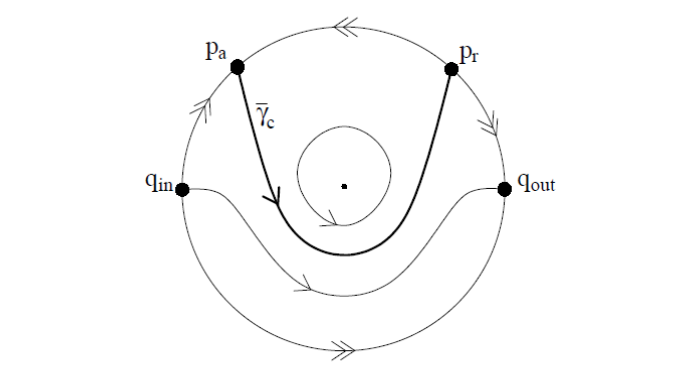
\includegraphics[height=6cm,width=10cm]{Images/CanardPointcircle}
%	\caption{The flow within our canard system \citep{krupa2001}.}
%	\label{fig: canard flow circle}
%\end{figure}\newpage
%where it is clear that our Hopf bifurcation is the periodic solution in the centre of Figure \ref{fig: canard flow circle} but we can see that below our special flow $ \bar{\gamma_c} $, our solution traverses through our equilbrium into our fast flow as we would expect in our original system.

%\newpage


\subsubsection{Separation of the Manifolds}\label{sec:separation-of-the-manifolds}
\begin{figure}[h!]\centering
	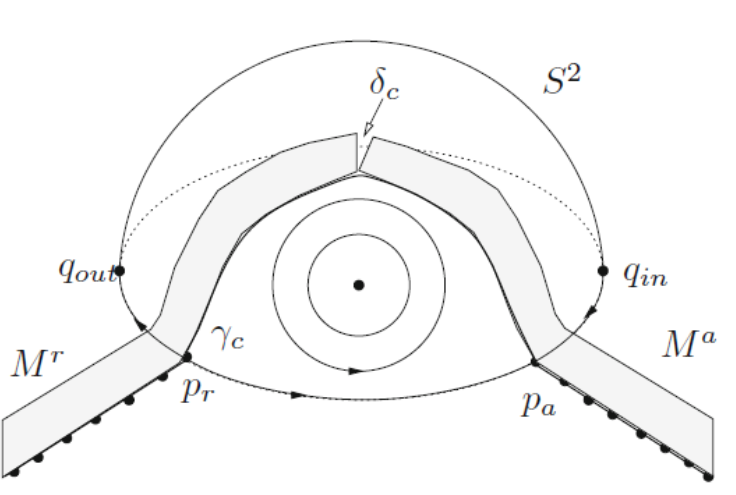
\includegraphics[height=8cm,width=10cm]{Images/Separation}
	\caption{Separation of $ M_a $ and $ M_r $ \citep{Kuehn}.}
	\label{fig: splitting}
\end{figure}%\newpage
%\textbf{Discuss splitting on the manifold}
Continuing on from the singular Hopf bifurcation we might find that the canard point forces our branches to split. In other words we are looking for when the attracting and repelling branches are no longer connected, as show in Figure \ref{fig: splitting}. To do this we would use Melnikov Computations to show that our manifolds split - see \textit{Extending Geometric Singular Perturbation Theory to Nonhyperbolic Points - Fold and Canard Points in Two Dimensions} \citep{krupa2001} for direct use. To discover whether we have a splitting between our branches we need to consider our $ y $ coordinates \wrt our second chart \st $ y_{a,2}(0)-y_{r,2}(0) $ is a distance function which can be written as $ D_c(r_2,\lambda_2)=H(0,y_{a,2}(0))-H(0,y_{r,2}(0)) $ as we note that $ \pd{}{y_2}H(0,y_2)\neq 0 $ \citep{krupa2001}. From here we can use the following proposition,
\begin{prop}
	[\citealp{krupa2001}]
	For a small enough $ \rho $ and $ \mu $ the distance function has the expansion
	\begin{equation*}
	D_c(r_2,\lambda_2)=d_{r_2}r_2+d_{\lambda_2}\lambda_2+O(2),
	\end{equation*}
	where we have defined,
	\begin{subequations}
		\begin{align}
		d_{r_2}&=\int_{-\infty}^{\infty}\text{grad}H(\gamma_{c,2}(t))^T\cdot G(\gamma_{c,2}(t))dt,\\
		d_{\lambda_2}&=\int_{-\infty}^{\infty}\text{grad}H(\gamma_{c,2}(t))^T\cdot (0,-1)^T,
		\end{align}
	\end{subequations}
	and our matrix $ G(\gamma_{c,2}(t)) $ in Section \ref{sec:dynamics-in-texorpdfstringk1k1} with $ \gamma_{c,2} $ as our critical trajectory. 
\end{prop}
Then, following the proof provided by \citet{krupa2001}, we find that we will have a split occurring between our branches if the canard falls outside of our domain of order $ O(e^{-\frac{c}{\epsilon}}) $ \st $ D_c(r_2,\lambda_2)\neq 0 $. We can calculate this explicitly for the the \vdp system by using Equations \ref{eq: const of motion}, \ref{eq: gamma c2} and $ G(x_2,y_2)=(-\frac{x_2^3}{3},0)^T $ \st we have,
\begin{subequations}
	\begin{align}
		d_{r_2}&=\int_{-\infty}^{\infty} \nabla\left(\frac{1}{2}e^{-2y_2}\left(y_2-x^2_2+\frac{1}{2}\right)\right)^T\cdot\left((-\frac{x_2^3}{3},0)^T\right)|_{\gamma_{c,2}} \text{dt}\\
%	&=\int_{-\infty}^{\infty}\left(-\frac{\exp\left(-\frac{t^2}{2}+1\right)}{2}.\frac{\exp\left(-\frac{t^2}{2}+1\right)}{2}\left(\frac{t^2}{4}-\frac{1}{2}-\frac{t}{2}\right)\right)
		&=
	\end{align}
\end{subequations}


 As a result of we see a flow similar to Figure \ref{fig: splitting} whereby we find that our flow could either jump off under the fast flow - see Figure \ref{fig: vdp flow diagram e} - or we might find that the flow could be trapped in the canard region and then be repelled back to the attracting manifold, as we see with our connected system - Figure \ref{fig: 4 canard }. 

\textbf{Good to have a figure if possible}




\newpage
\appendix
\section{Dynamics in \texorpdfstring{$K_2$}{K2}}

\newpage
\bibliography{FastSlow.bib}
\bibliographystyle{agsm}
\nocite{strogatz2007nonlinear}
\appendix
\section{Log}
\end{document}
